% =============================================================================
%  PTHSonde -- Radiosonde System: User Manual & Operations Guide
%  Tracer Lab
%
%  Copy this whole file into Overleaf. Also upload the "assets/" folder
%  (the images referenced below) alongside this main.tex.
%  Compiler: pdfLaTeX.
% =============================================================================
\documentclass[11pt,openany]{report}

\usepackage[a4paper,margin=1in]{geometry}
\usepackage[T1]{fontenc}
\usepackage{lmodern}
\usepackage{graphicx}
\usepackage[table]{xcolor}
\usepackage{tikz}
\usetikzlibrary{shapes.geometric,arrows.meta,positioning,calc,fit,backgrounds}
\usepackage{booktabs}
\usepackage{array}
\usepackage{enumitem}
\usepackage{caption}
\usepackage{float}
\usepackage{amsmath}
\usepackage{fancyhdr}
\usepackage{titlesec}
\usepackage[most]{tcolorbox}
\usepackage[hidelinks]{hyperref}

\graphicspath{{assets/}}

% ---- Brand colors ----------------------------------------------------------
\definecolor{tlorange}{RGB}{239,127,26}
\definecolor{tldark}{RGB}{26,28,33}
\definecolor{tlgray}{RGB}{90,96,104}
\definecolor{tllight}{RGB}{245,246,248}
\definecolor{tlblue}{RGB}{52,120,200}

% ---- Section styling -------------------------------------------------------
\titleformat{\chapter}[display]
  {\normalfont\huge\bfseries\color{tldark}}
  {\color{tlorange}\Large\MakeUppercase{\chaptertitlename}\ \thechapter}{8pt}{\Huge}
\titlespacing*{\chapter}{0pt}{-10pt}{24pt}
\titleformat{\section}{\normalfont\Large\bfseries\color{tldark}}{\color{tlorange}\thesection}{0.6em}{}
\titleformat{\subsection}{\normalfont\large\bfseries\color{tldark}}{\color{tlorange}\thesubsection}{0.6em}{}

% ---- Header / footer -------------------------------------------------------
\pagestyle{fancy}
\fancyhf{}
\renewcommand{\headrulewidth}{0.4pt}
\renewcommand{\headrule}{\hbox to\headwidth{\color{tlorange}\leaders\hrule height \headrulewidth\hfill}}
\fancyhead[L]{\footnotesize\color{tlgray}\textbf{PTH}\textcolor{tlorange}{\textbf{Sonde}}}
\fancyhead[R]{\footnotesize\color{tlgray}User Manual \& Operations Guide}
\fancyfoot[C]{\thepage}
\fancyfoot[R]{\footnotesize\color{tlgray}Tracer Lab}

% ---- Callout boxes ---------------------------------------------------------
\newtcolorbox{tip}{colback=tlorange!8,colframe=tlorange,boxrule=0.8pt,arc=3pt,
  left=8pt,right=8pt,top=6pt,bottom=6pt,fonttitle=\bfseries,title={\raggedright Tip}}
\newtcolorbox{warn}{colback=red!5,colframe=red!70!black,boxrule=0.8pt,arc=3pt,
  left=8pt,right=8pt,top=6pt,bottom=6pt,fonttitle=\bfseries,title={\raggedright Caution}}
\newtcolorbox{note}{colback=tlblue!6,colframe=tlblue,boxrule=0.8pt,arc=3pt,
  left=8pt,right=8pt,top=6pt,bottom=6pt,fonttitle=\bfseries,title={\raggedright Note}}

\captionsetup{font=small,labelfont={bf,color=tlorange}}
\setlist{itemsep=2pt,topsep=3pt}
\newcommand{\PTH}{\texorpdfstring{\textbf{PTH}\textcolor{tlorange}{\textbf{Sonde}}}{PTHSonde}}
\raggedbottom  % don't stretch pages vertically -> avoids big blank gaps around figures

% =============================================================================
\begin{document}

% ------------------------------- TITLE PAGE ---------------------------------
\begin{titlepage}
\thispagestyle{empty}
% severe-weather backdrop (NOAA cumulonimbus, public domain)
\begin{tikzpicture}[remember picture,overlay]
  \node[inner sep=0] at (current page.center)
    {
\includegraphics[width=\paperwidth,height=\paperheight]{title_bg.png}};
\end{tikzpicture}%
\centering
\vspace*{0.5cm}


\includegraphics[width=0.52\textwidth]{logo_pthsonde.png}\\[0.7cm]

{\color{tlorange}\rule{0.72\textwidth}{2pt}}\\[0.35cm]
{\Huge\bfseries\color{tldark} Radiosonde System}\\[0.22cm]
{\LARGE\color{tlgray} User Manual \& Operations Guide}\\[0.30cm]
{\color{tlorange}\rule{0.72\textwidth}{2pt}}\\[0.7cm]

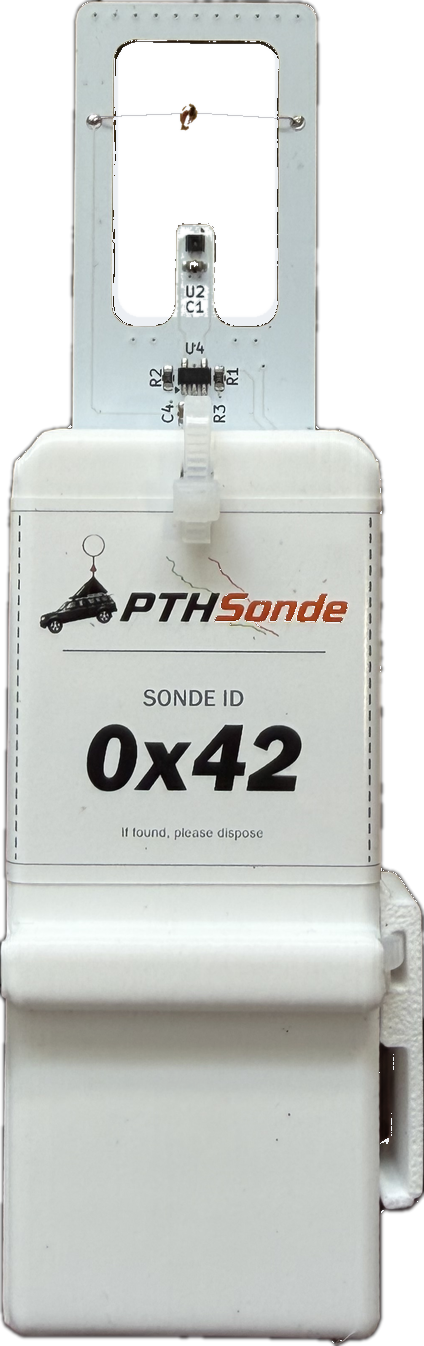
\includegraphics[height=0.44\textheight]{sonde_hero.png}\\[0.5cm]

\vfill

\includegraphics[width=0.30\textwidth]{logo_tracerlab.png}\\[0.5cm]
{\color{tlgray}\small Document revision 1.0 \quad\textbullet\quad \today}
\end{titlepage}

\tableofcontents
\clearpage

% =============================================================================
\chapter*{Safety \& Regulatory Notice}
\addcontentsline{toc}{chapter}{Safety \& Regulatory Notice}

\begin{warn}
\textbf{Read this before you fly.} Launching a free balloon puts hardware into shared
airspace. \textbf{You, the operator, are solely responsible for conducting every flight
safely and legally.}
\end{warn}

\vspace{4pt}
\noindent Before and during every flight it is \textbf{your responsibility} to:

\begin{itemize}
  \item \textbf{Know and follow all applicable laws and regulations} for your location
        --- national aviation authority rules (e.g.\ in the United States, FAA
        regulations on unmanned free balloons), airspace restrictions, notification
        requirements, payload-weight limits, and any local ordinances.
  \item \textbf{Check the airspace} you will fly through and avoid controlled,
        restricted, or prohibited areas. Coordinate with or notify air-traffic
        authorities where required, and never launch near airports or active flight
        corridors.
  \item \textbf{Assess the conditions and recovery area} --- weather, wind, predicted
        landing zone, terrain, people, property, roads, power lines and water --- and
        launch only when it is safe to do so.
  \item \textbf{Handle the gas safely.} Helium and especially hydrogen require correct
        handling; hydrogen is flammable. Follow all gas-supplier and safety guidance.
\end{itemize}

\vspace{4pt}
\noindent
\textbf{Assumption of risk and no liability.} The \PTH{} is provided \emph{as is}, for
research, educational, operational and hobby use. The designers, manufacturers, contributors and
suppliers of the \PTH{} and this manual accept \textbf{no liability whatsoever} for any
loss, damage, injury, regulatory violation or other consequence arising from its use.
By building, launching or operating a \PTH{}, \textbf{you accept full responsibility}
for doing so lawfully and safely, and you assume all associated risk. If you are unsure
whether a flight is legal or safe, \textbf{do not launch.}

\clearpage

% =============================================================================
\chapter{System Overview}

The \PTH{} is a complete radiosonde system: a small, reusable weather-balloon
payload that measures \textbf{P}ressure, \textbf{T}emperature and \textbf{H}umidity
(plus wind, GPS position and battery health), streams it to the ground over a
long-range 915\,MHz LoRa link, and displays it live in a one-click desktop
ground station that renders a full SHARPpy atmospheric sounding.

\section{How the system fits together}
The system has four parts: the sonde in the air, the radio link, the ground
receiver, and the dashboard.

\begin{figure}[htbp]
\centering
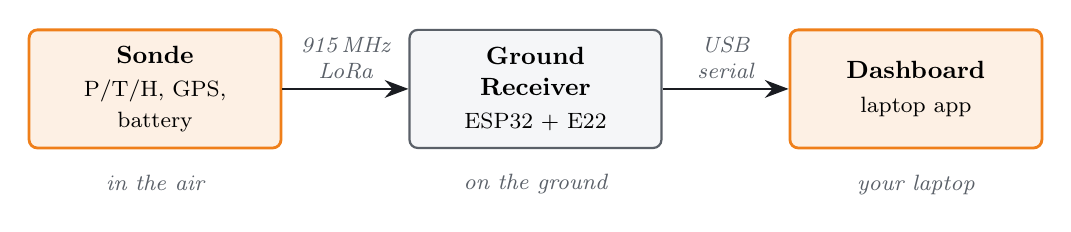
\begin{tikzpicture}[
  node distance=10mm and 16mm,
  box/.style={rounded corners=3pt,draw=tlgray,line width=0.8pt,fill=tllight,
              minimum width=32mm,minimum height=15mm,align=center,font=\small},
  acc/.style={box,fill=tlorange!12,draw=tlorange,line width=1pt},
  lbl/.style={font=\footnotesize\itshape,color=tlgray},
  arr/.style={-{Stealth[length=3mm]},line width=1pt,color=tldark}]

  \node[acc] (sonde) {\textbf{Sonde}\\[1pt]\footnotesize P/T/H, GPS,\\\footnotesize battery};
  \node[box,right=of sonde] (rx) {\textbf{Ground}\\\textbf{Receiver}\\[1pt]\footnotesize ESP32 + E22};
  \node[acc,right=of rx] (dash) {\textbf{Dashboard}\\[1pt]\footnotesize laptop app};

  \draw[arr] (sonde) -- node[lbl,above,align=center]{915\,MHz\\LoRa} (rx);
  \draw[arr] (rx) -- node[lbl,above,align=center]{USB\\serial} (dash);

  \node[lbl,below=2mm of sonde,align=center]{in the air};
  \node[lbl,below=2mm of rx,align=center]{on the ground};
  \node[lbl,below=2mm of dash,align=center]{your laptop};
\end{tikzpicture}
\caption{The \PTH{} signal chain: the airborne sonde transmits telemetry over LoRa to a
ground receiver, which forwards it over USB to the desktop dashboard.}
\end{figure}

\section{Key features}
\begin{itemize}
  \item \textbf{Long-range LoRa} --- Ebyte E22 at 22\,dBm / 0.3\,kbps air rate for maximum link margin.
  \item \textbf{Barometric flight data} --- altitude, ascent rate and the sounding are derived
        from the pressure sensor, so they remain valid above the GPS ceiling.
  \item \textbf{SHARPpy analysis} --- an SPC-style Skew-T and index panel rendered from each flight.
  \item \textbf{Reusable payload} --- a 3D-printed enclosure with a swappable battery; recover it and fly again.
  \item \textbf{Per-unit identity} --- each sonde derives a stable hex ID from its chip, printed on its sticker.
\end{itemize}

\begin{note}
This guide covers the full operational workflow: preparing the sonde, pairing it
with the ground station, filling the balloon, launching, and analysing the flight.
It assumes the firmware is already flashed and the desktop app installed.
\end{note}

% =============================================================================
\chapter{The Sonde}

The \PTH{} payload (shown on the cover) is a single ESP32-C3 board carrying the
sensor suite and the radio, housed in a lightweight, reusable 3D-printed shell with
a removable battery door and an exposed thermistor probe for true air temperature.

\section{Measurement specifications}
The \PTH{} measures the full \textbf{P}ressure / \textbf{T}emperature /
\textbf{H}umidity state of the air, plus wind and position. The table below gives the
rated performance of each measurement over the operating envelope.

\begin{table}[H]
\centering\small
\setlength{\tabcolsep}{6pt}
\renewcommand{\arraystretch}{1.35}
\begin{tabular}{@{}>{\bfseries}l l l l l@{}}
\toprule
\rowcolor{tlorange!22}
\textbf{Parameter} & \textbf{Range} & \textbf{Accuracy} & \textbf{Resolution} & \textbf{Response ($\tau_{63}$)} \\
\midrule
Air temperature & $-70$ to $+50\,^\circ$C & $\pm0.3\,^\circ$C & $0.01\,^\circ$C & $<2$\,s \\
\rowcolor{tllight}
Relative humidity & $0$--$100\,\%$RH & $\pm1.8\,\%$RH & $0.1\,\%$RH & $\sim4$\,s \\
Barometric pressure & $10$--$1200$\,hPa & $\pm1.5$\,hPa & $0.01$\,hPa & $<20$\,ms \\
\rowcolor{tllight}
Pressure altitude (derived) & $0$--$12$\,km & $\pm10$\,m & $1$\,m & $<1$\,s \\
Wind speed & $0$--$90$\,m/s & $\pm0.5$\,m/s & $0.1$\,m/s & $1$\,s (1\,Hz) \\
\rowcolor{tllight}
Wind direction & $0$--$360^\circ$ & $\pm5^\circ$ & $1^\circ$ & $1$\,s (1\,Hz) \\
GPS position & global & $\pm2.5$\,m CEP & --- & $1$\,s (1\,Hz) \\
\bottomrule
\end{tabular}
\caption{Rated measurement performance of the \PTH{} sensor suite.}
\end{table}

\begin{note}
\textbf{Operating envelope: surface to 12\,km.} The \PTH{} is rated from the ground
through the boundary layer and into the lower and middle troposphere --- the altitudes
that matter for boundary-layer research, convective profiling, and lower/mid-tropospheric
soundings. Temperature is measured by a fast, directly-exposed bead thermistor for true
air temperature; humidity and pressure are sensed by dedicated digital sensors; wind is
derived at 1\,Hz from the GPS track.
\end{note}

\section{The flight train mass}
The complete flight train --- the \PTH{} in its enclosure, battery, sticker and the
line hardware that connects it to the balloon --- is designed to weigh about
\textbf{80\,grams} total. This is the payload mass used for all the balloon
calculations in Chapter~5.

% =============================================================================
\chapter{Preparing the Sonde for Flight}

Before every flight the sonde needs a fresh battery, the door secured, and the
payload tied onto the flight line. The three steps below take about two minutes.

\section{Step 1 --- Insert the battery}
Open the outer battery door and slide the cell into the holder, observing the
polarity marked inside the bay. The board powers up immediately and begins its
boot self-test.

\begin{note}
\textbf{Recommended battery: Energizer Lithium CR123.} This lithium cell is the
right choice for the \PTH{} --- it is light, holds a high energy density, and
(critically) keeps delivering current in the extreme cold of the stratosphere,
where ordinary alkaline cells sag and die. Always fly a fresh CR123.
\end{note}

\begin{figure}[htbp]
\centering
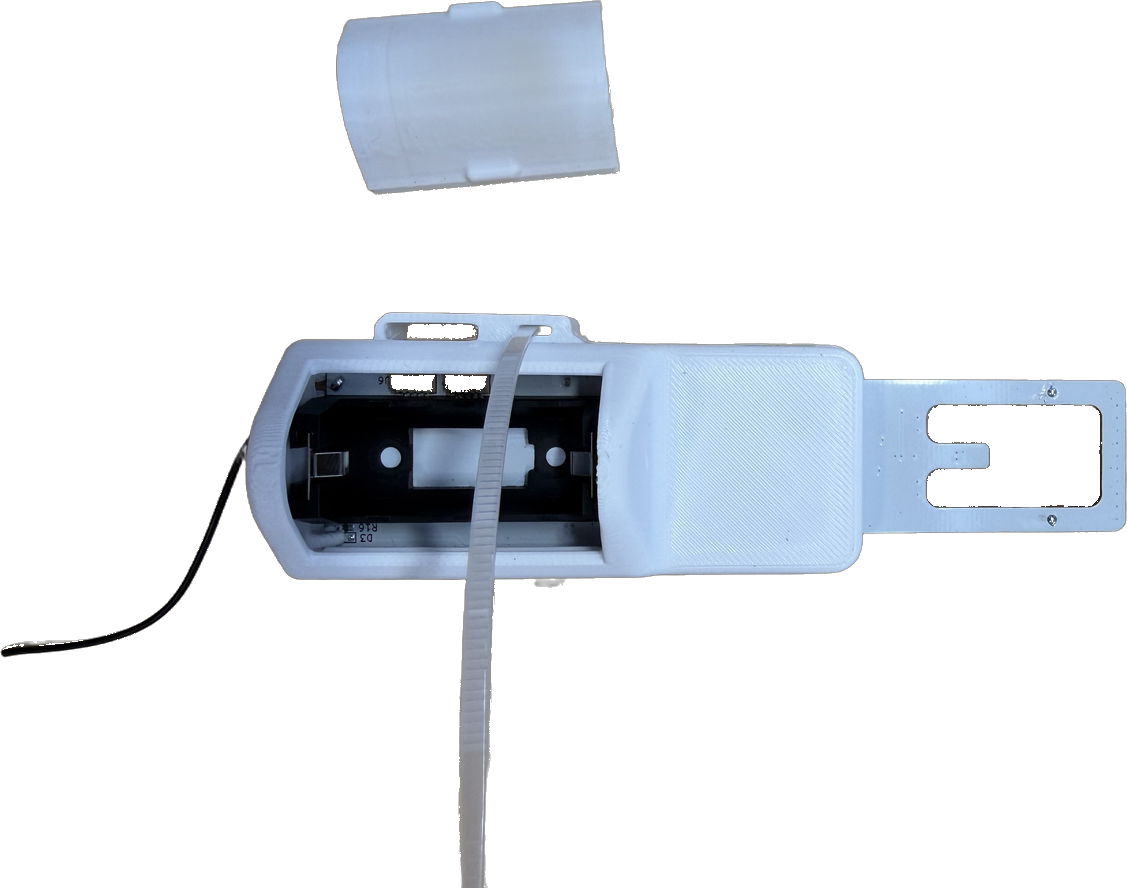
\includegraphics[width=0.92\textwidth]{sonde_battery.png}
\caption{The open battery bay. Insert the cell into the holder (centre), minding polarity.
The mounting bracket is on the right; the zip tie (left) will secure the outer door.}
\end{figure}

\begin{tip}
On power-up the status LED blinks while the radio and GPS initialise. If you have
the sonde on USB, it prints its \textbf{Sonde ID} and a per-sensor health line ---
confirm every sensor reads \texttt{ok} before you close it up.
\end{tip}

\section{Step 2 --- Close and zip-tie the door}
Refit the outer battery door and lock it down with a zip tie through the retaining
slots. This keeps the battery seated through the launch and the landing.

\begin{figure}[htbp]
\centering
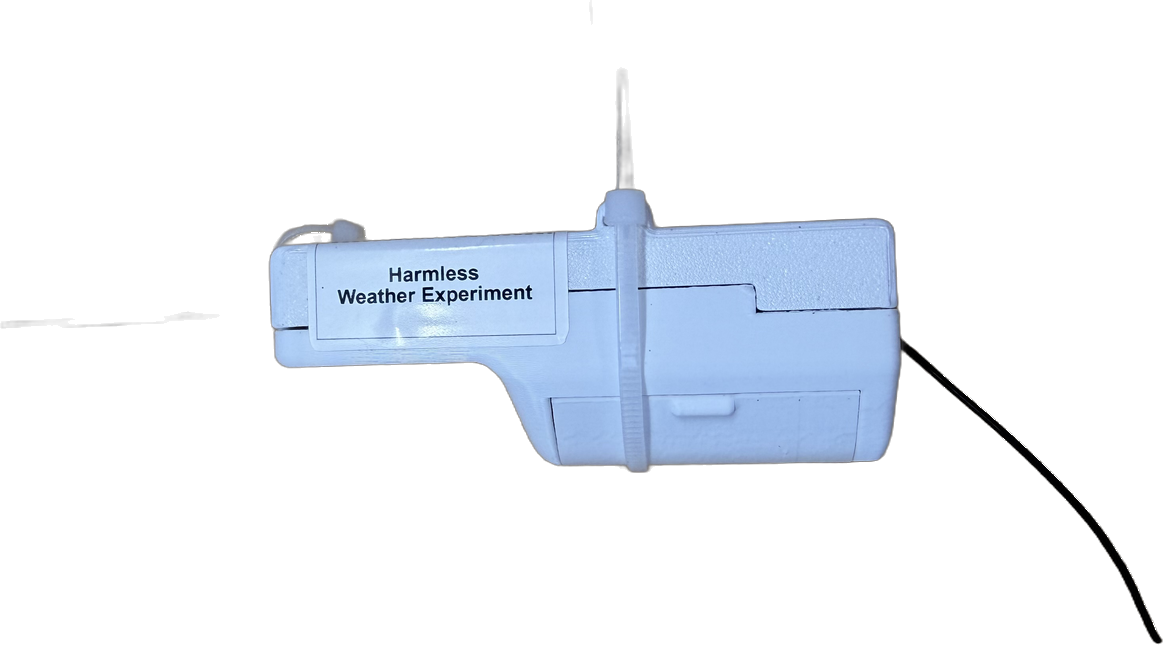
\includegraphics[width=0.72\textwidth]{sonde_ziptie.png}
\caption{The closed enclosure with the outer door zip-tied shut. The printed sticker carries
the sonde's hex ID and the finder instructions.}
\end{figure}

\section{Step 3 --- Tie the sonde to the flight line}
Thread the flight line through the bracket and tie it off so the payload hangs
cleanly below the parachute. Use a strong, non-slip knot; this single line carries
the payload for the whole flight.

\begin{warn}
Do not launch with a loose or frayed line. The knot at the bracket is the only
thing holding your payload to the balloon --- inspect it before every flight.
\end{warn}

\begin{figure}[htbp]
\centering
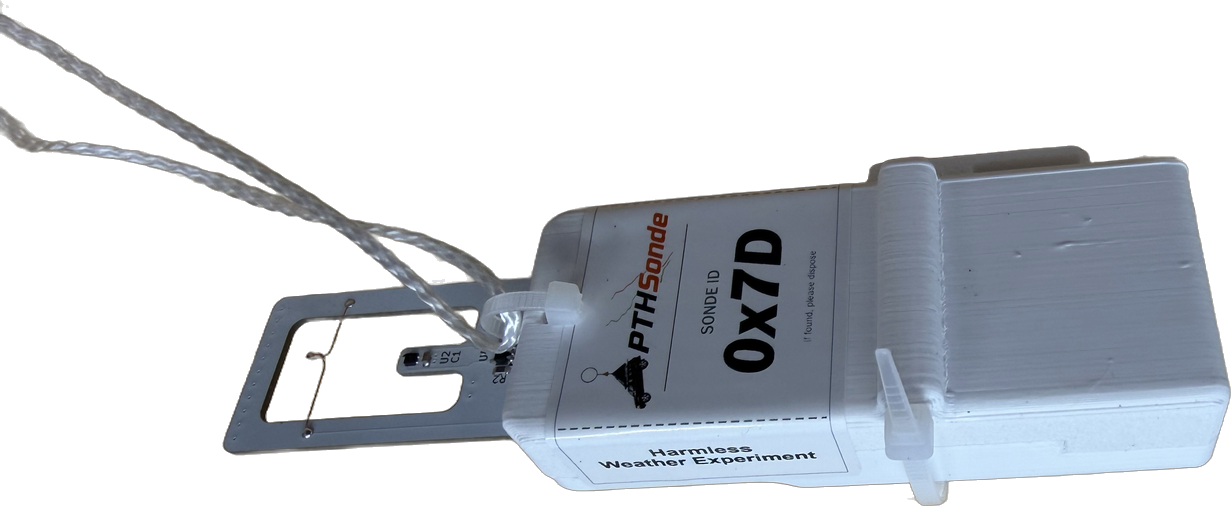
\includegraphics[width=0.86\textwidth]{sonde_flightline.png}
\caption{The finished sonde tied onto the flight line, ready to be attached below the
parachute and balloon. Note the exposed thermistor board (left) that reads the true air temperature.}
\end{figure}

% =============================================================================
\chapter{The Ground Station \& Dashboard}

The ground station is a one-window desktop app. It owns the USB serial port to the
receiver, records the flight, and draws everything live --- telemetry, a Skew-T,
a hodograph, time-series, a landing-prediction map, and the SHARPpy panel.

\section{The ground receiver and antenna}
The receiver is a small 3D-printed box housing an ESP32 with the same E22 LoRa radio
as the sonde, an SMA antenna connector, and a USB lead to your laptop. Like the
sonde, each receiver carries its own hex ID on a printed sticker.

\begin{figure}[htbp]
\centering
\rotatebox{180}{
\includegraphics[height=0.58\textheight]{gcs.png}}
\caption{The ground station: the receiver box (here \emph{Ground Station 0x74}), its
magnetic-mount 915\,MHz whip antenna, and the USB lead to the laptop.}
\end{figure}

\begin{tip}
\textbf{Antenna placement is the single biggest factor in your range.} Give the
antenna a clear, unobstructed \emph{view of the sky}, and mount it \emph{as high as
possible} --- away from buildings, vehicles and metal, ideally on a mast, a rooftop,
or a magnetic roof mount. The higher and clearer the
antenna, the longer you hold the link as the balloon drifts toward the horizon.
\end{tip}

\section{Pairing the sonde with the ground station}
\begin{enumerate}
  \item Plug the ground receiver into your laptop over USB and launch the dashboard
        (the truck icon).
  \item In the top bar, select the receiver's \textbf{COM port} and press
        \textbf{Connect}. The link indicator turns live and packets begin to count up.
  \item Power on the sonde. Within a few seconds its \textbf{Sonde ID} appears in
        the left-hand \textsc{Link} panel and the sensor dots at the bottom light green.
  \item Use the channel controls to \textbf{stage} and, at launch, \textbf{lock} the
        sonde onto your flight frequency.
\end{enumerate}

\begin{figure}[htbp]
\centering
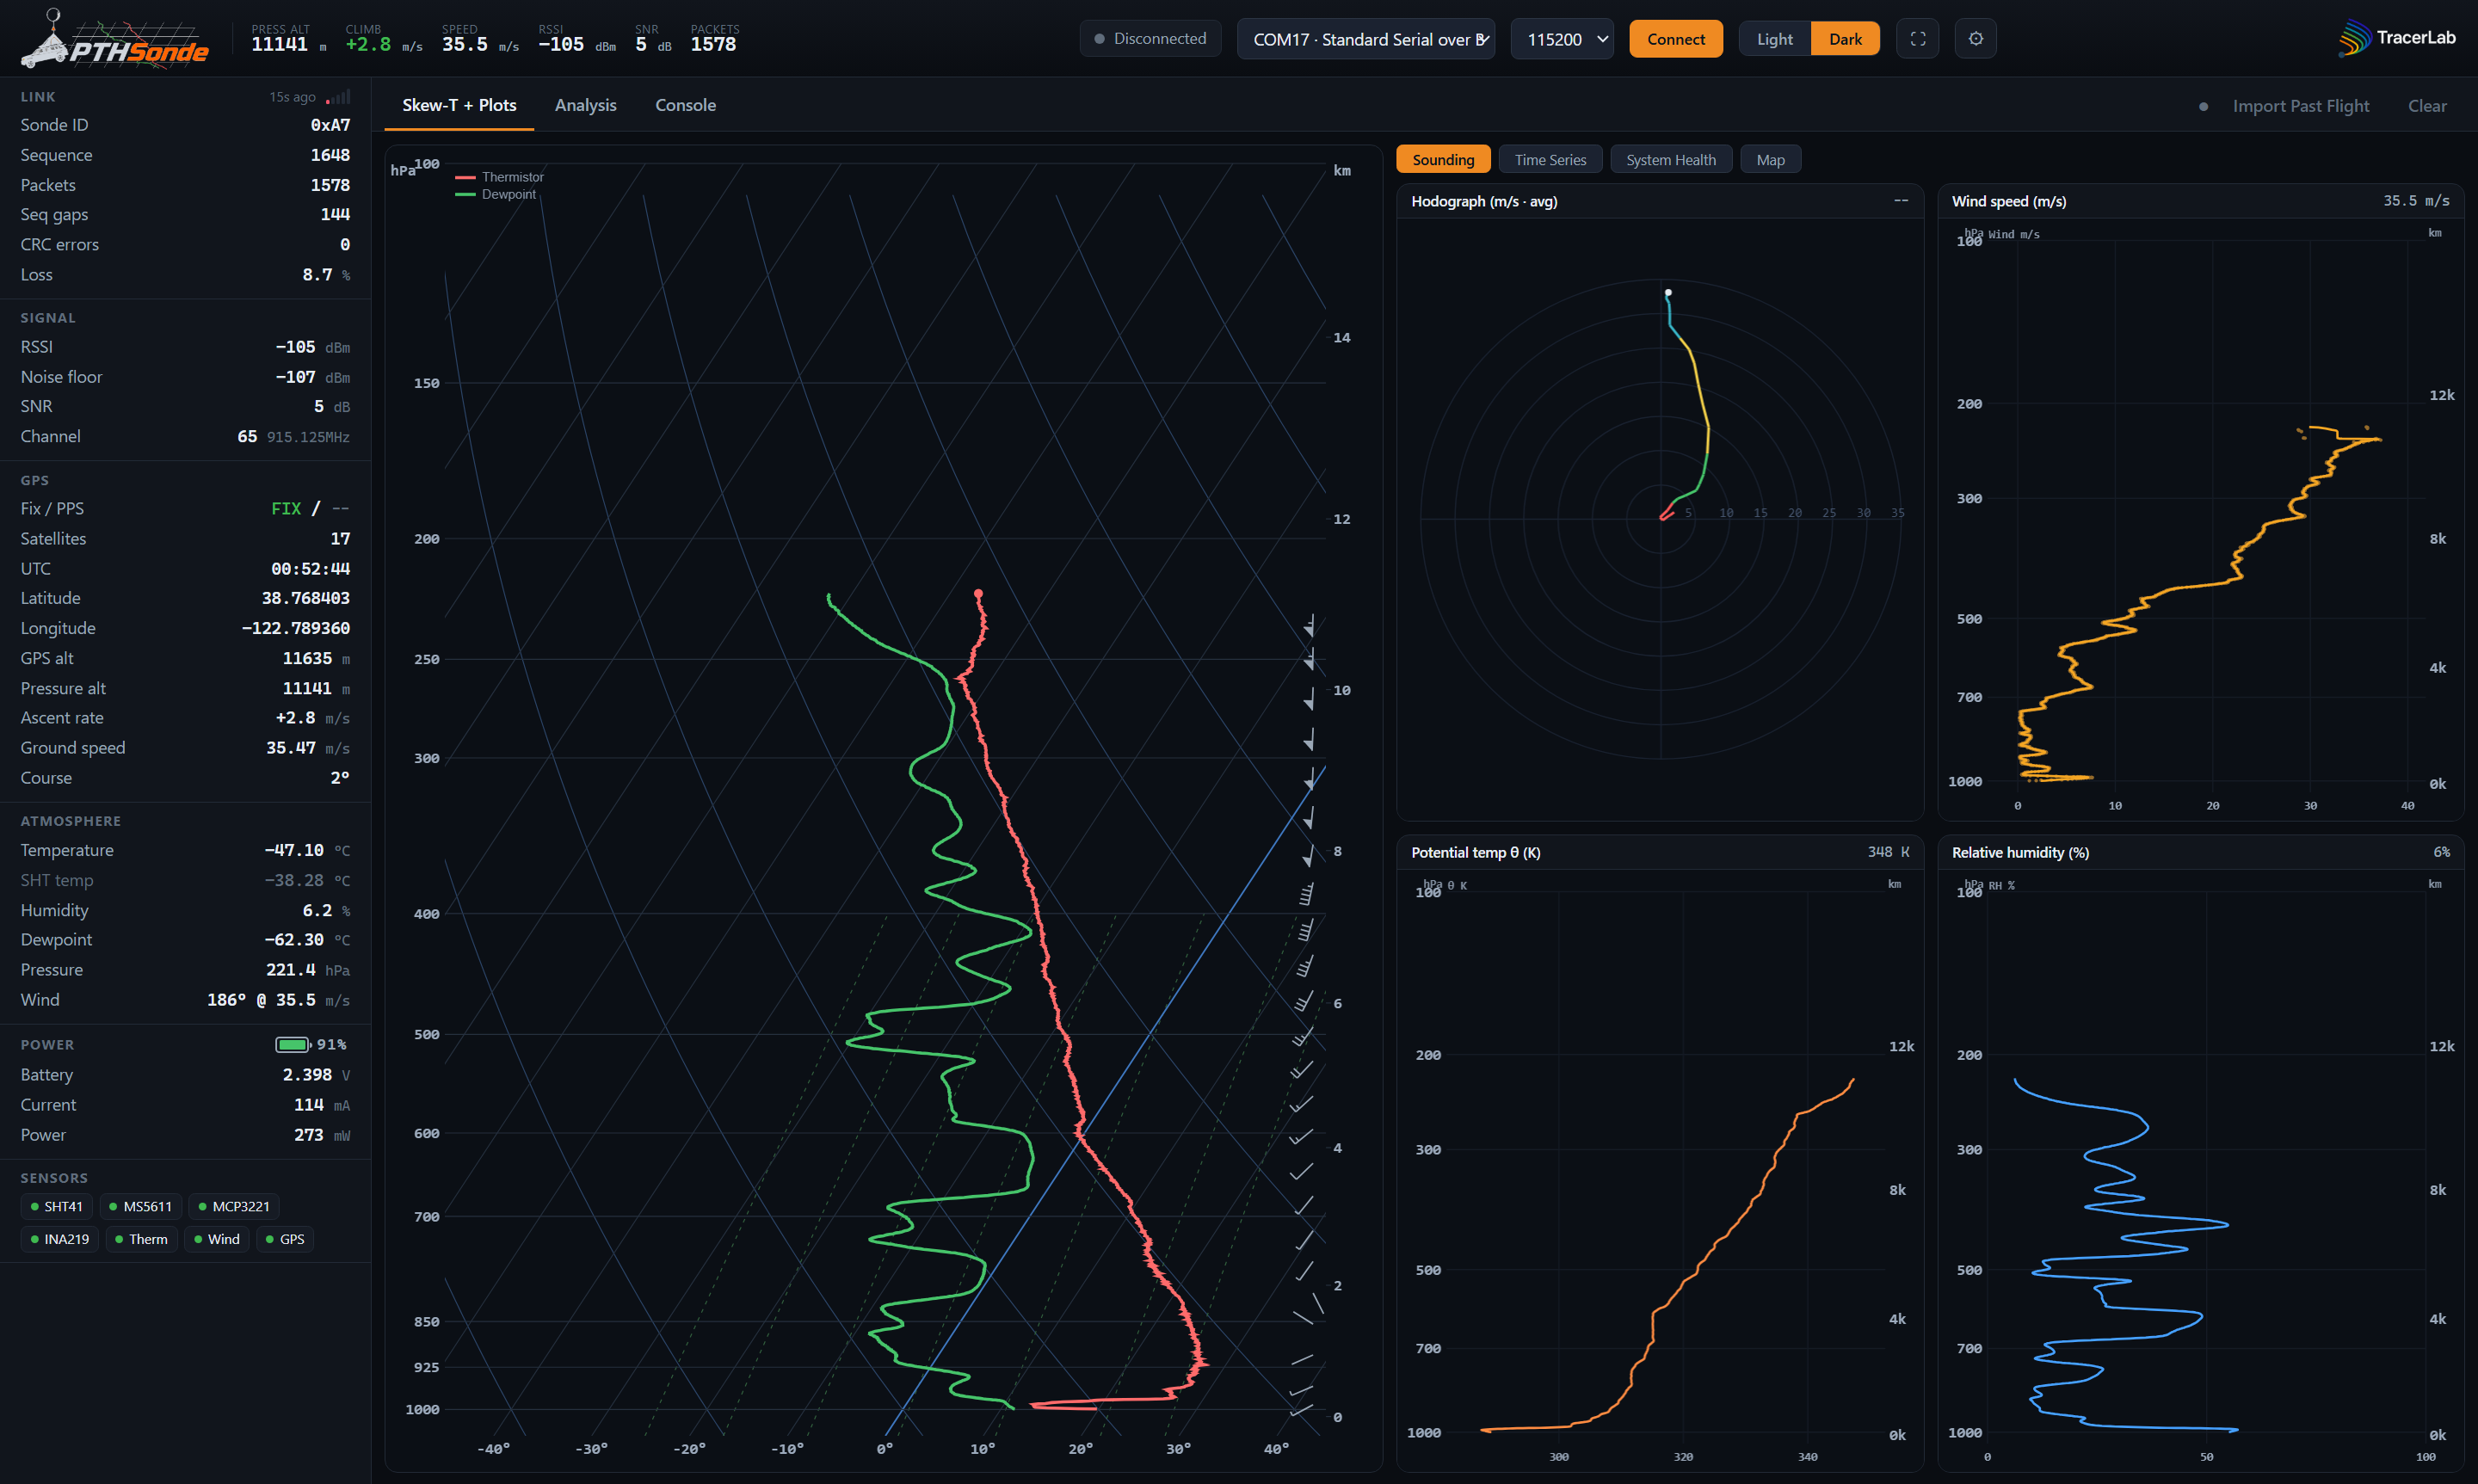
\includegraphics[width=\textwidth]{dash_profile.png}
\caption{The live dashboard during a flight. Left: link, signal, GPS, atmosphere, power and
per-sensor health. Centre: the Skew-T with the thermistor (red) and dewpoint (green) traces and
wind barbs. Right: hodograph, wind-speed, potential-temperature and relative-humidity profiles.}
\end{figure}

\begin{note}
The header strip shows the headline numbers at a glance: pressure altitude, climb
rate, ground speed, link RSSI/SNR and packet count. The connect controls and
light/dark theme toggle live on the right.
\end{note}

\section{Reading the panels}
The right pane switches between four views.

\begin{figure}[htbp]
\centering
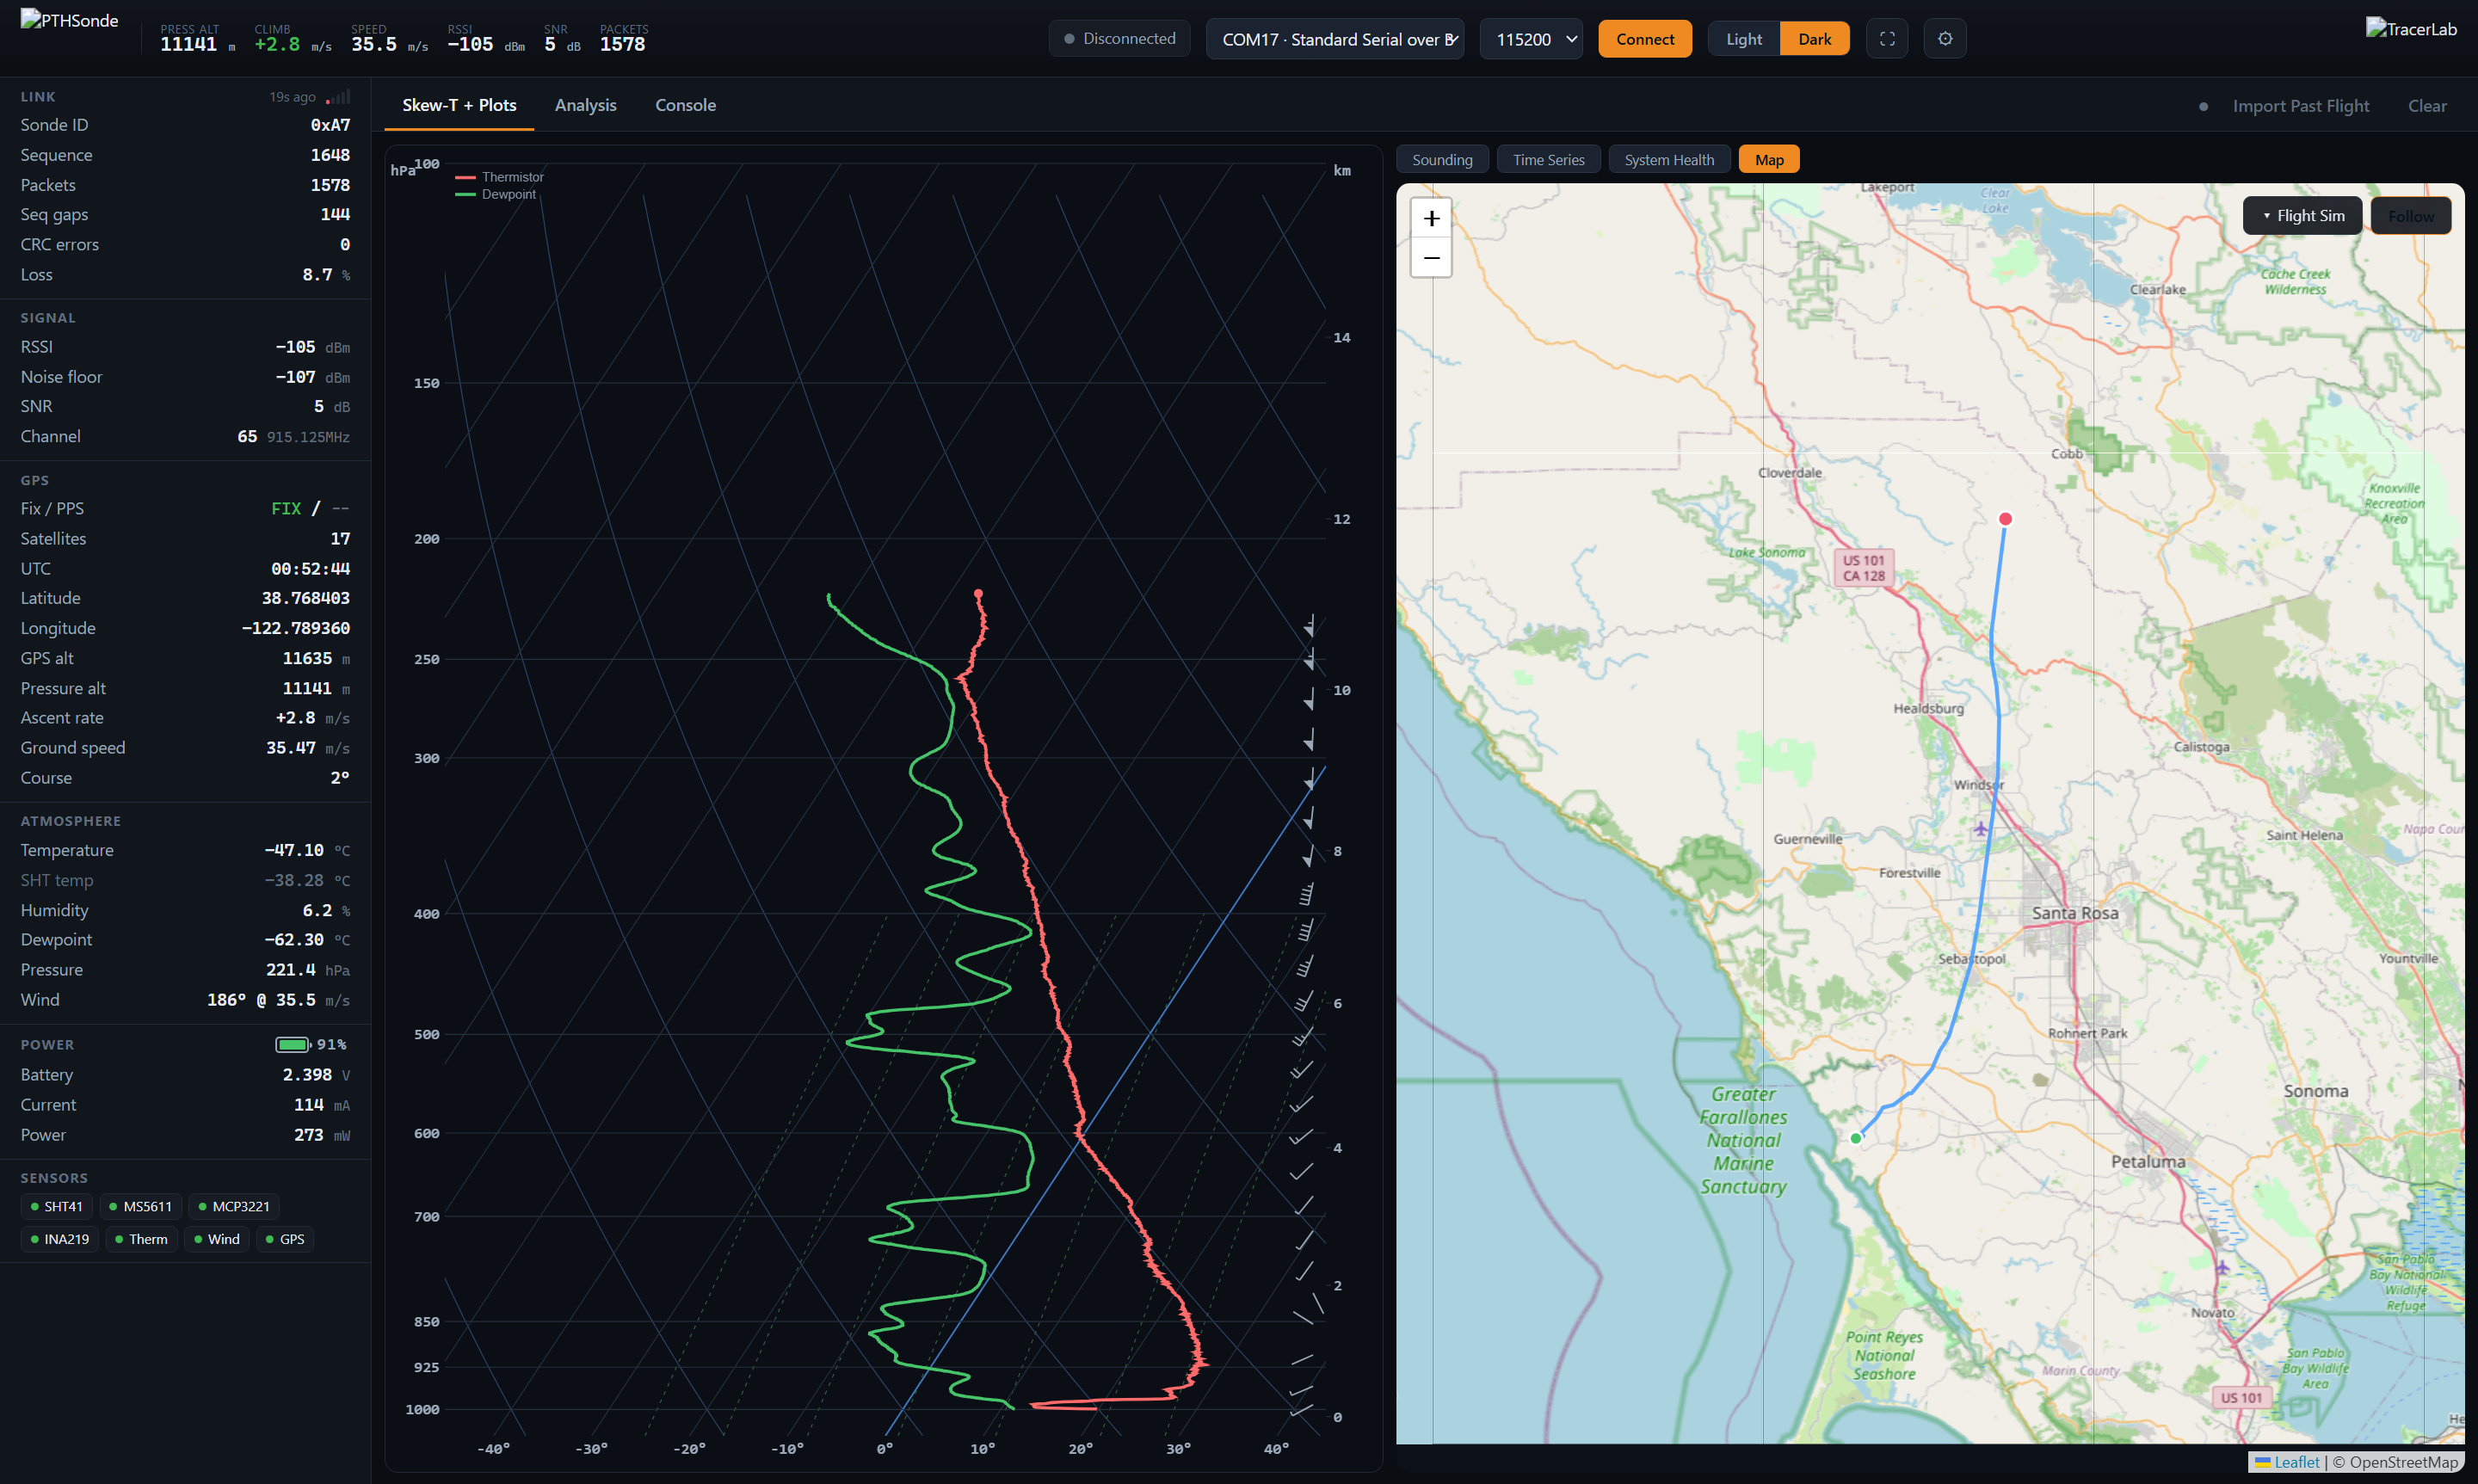
\includegraphics[width=\textwidth]{dash_map.png}
\caption{\textbf{Map} view --- the live position and predicted landing overlaid on the terrain,
so you can drive to the recovery point while the sonde is still flying.}
\end{figure}

\begin{figure}[htbp]
\centering
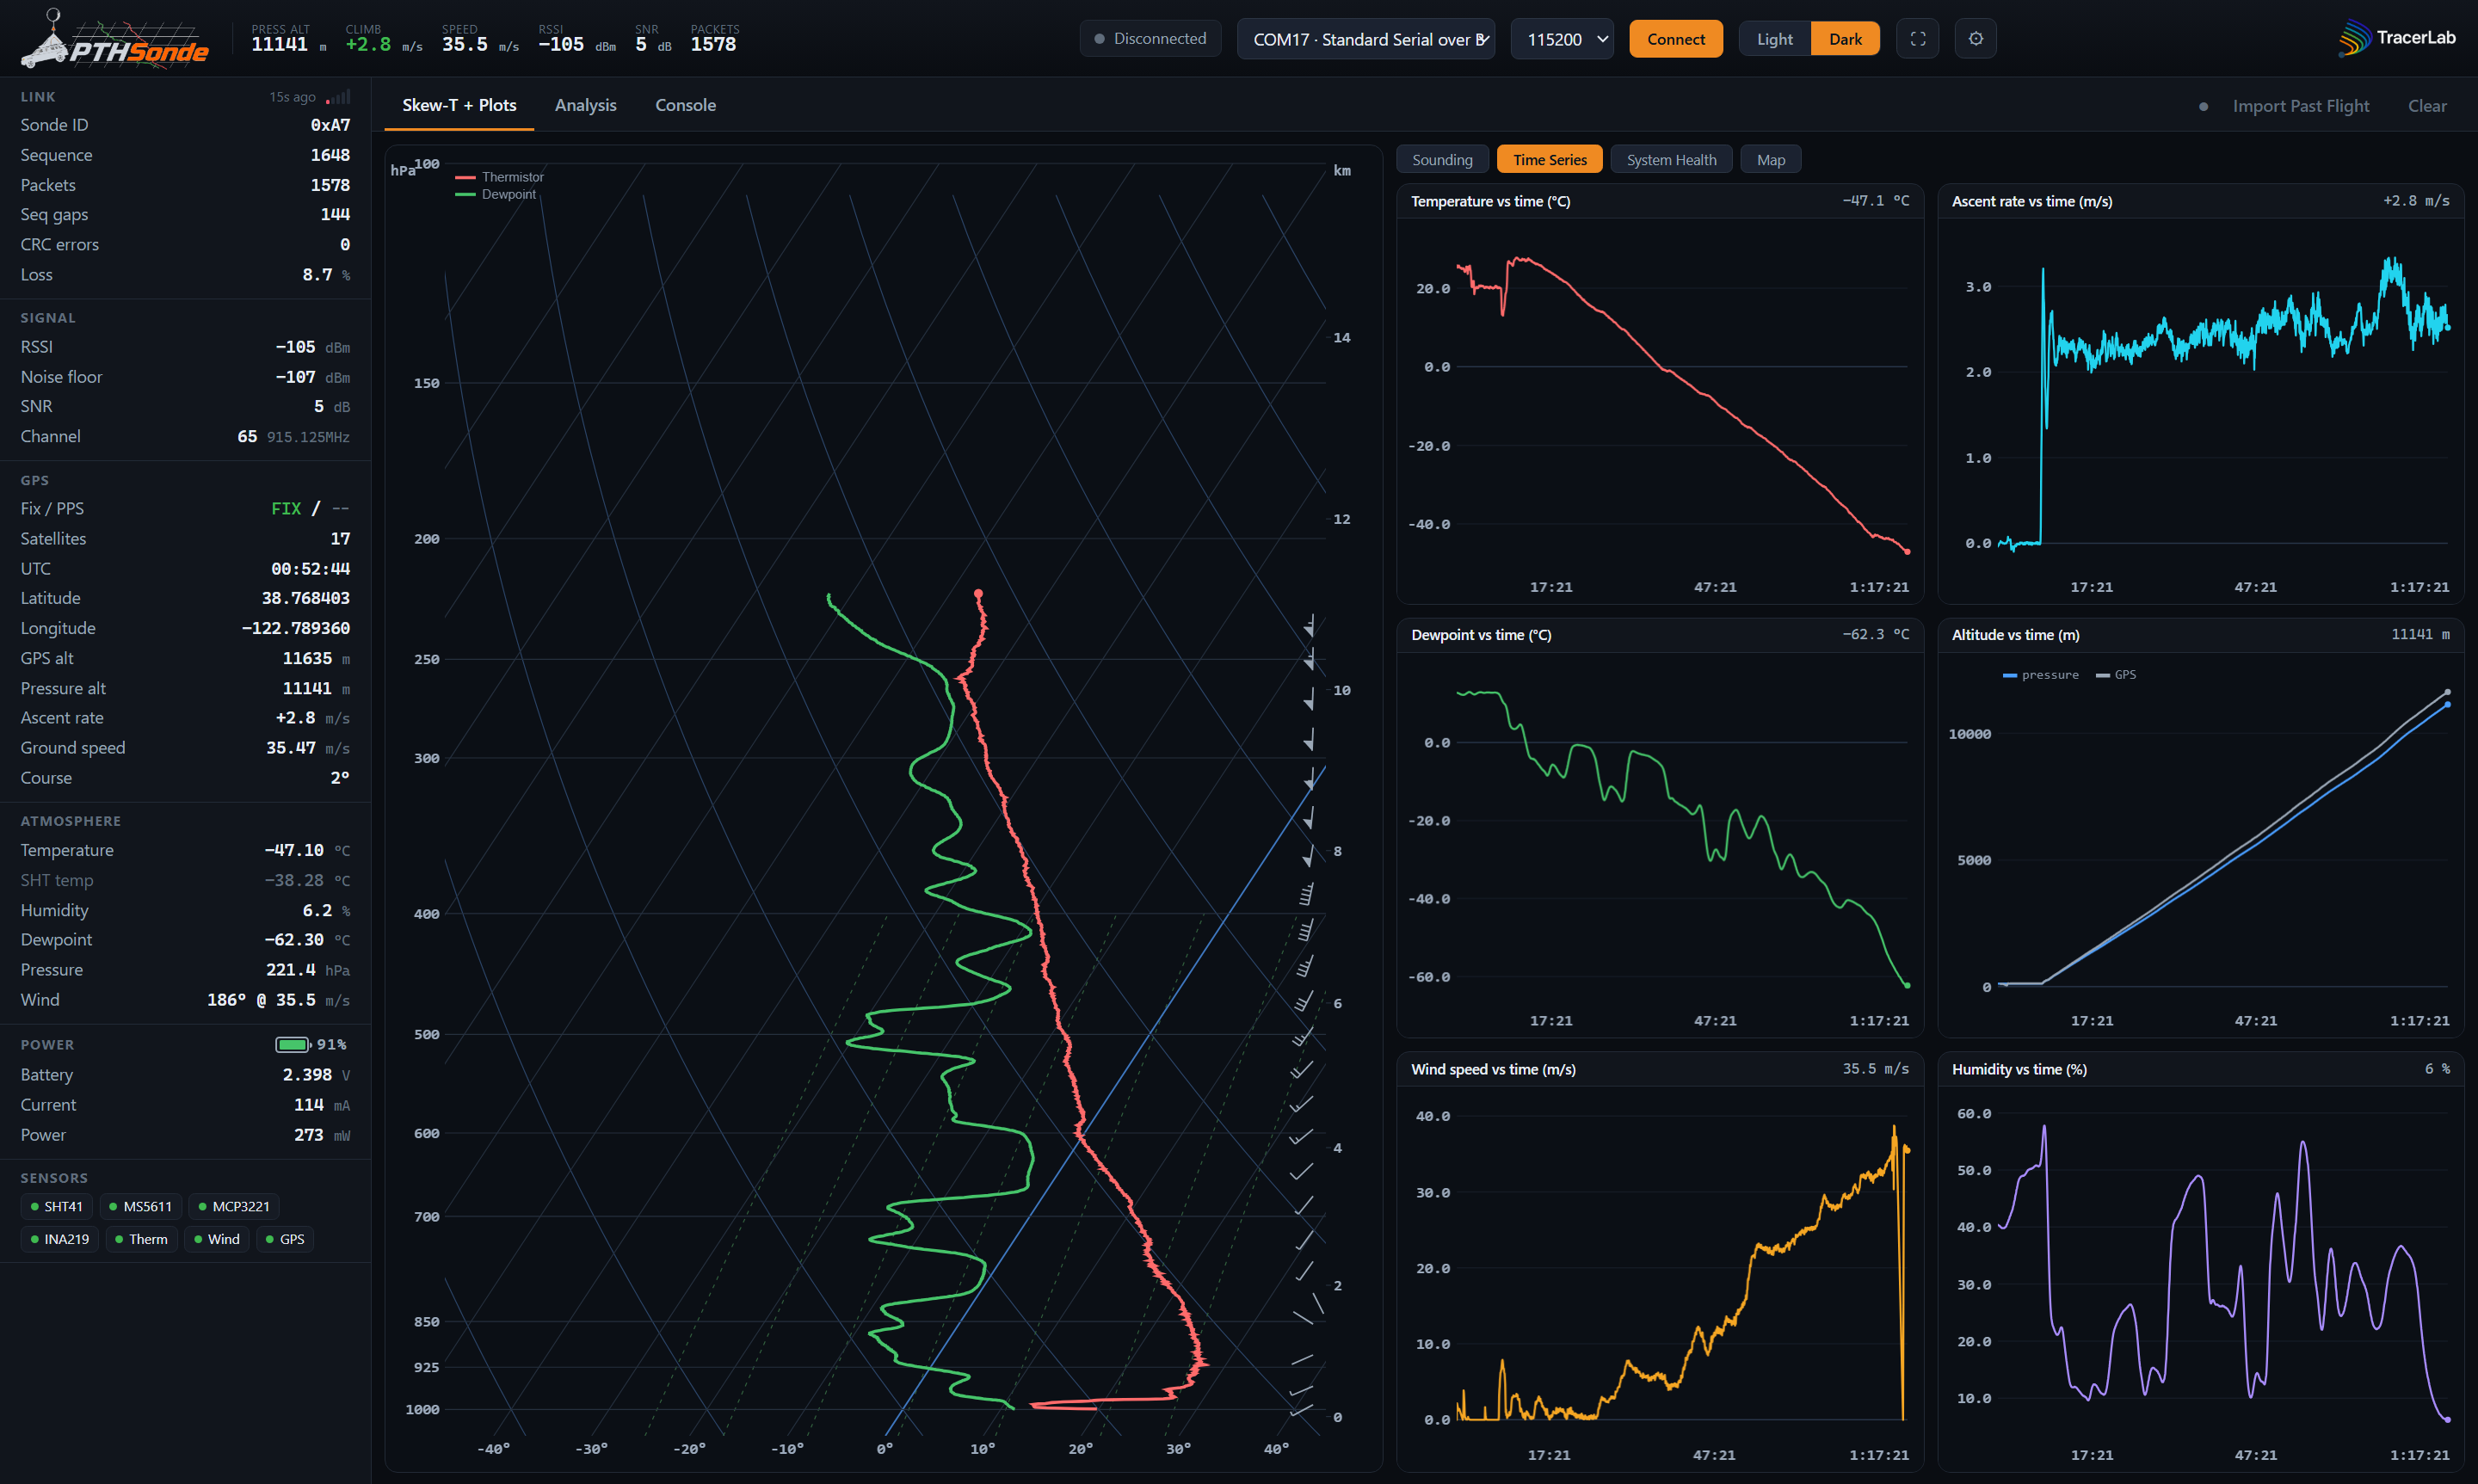
\includegraphics[width=\textwidth]{dash_timeseries.png}
\caption{\textbf{Time Series} view --- every channel plotted against time for a quick
sanity check of the whole flight.}
\end{figure}

\begin{figure}[htbp]
\centering
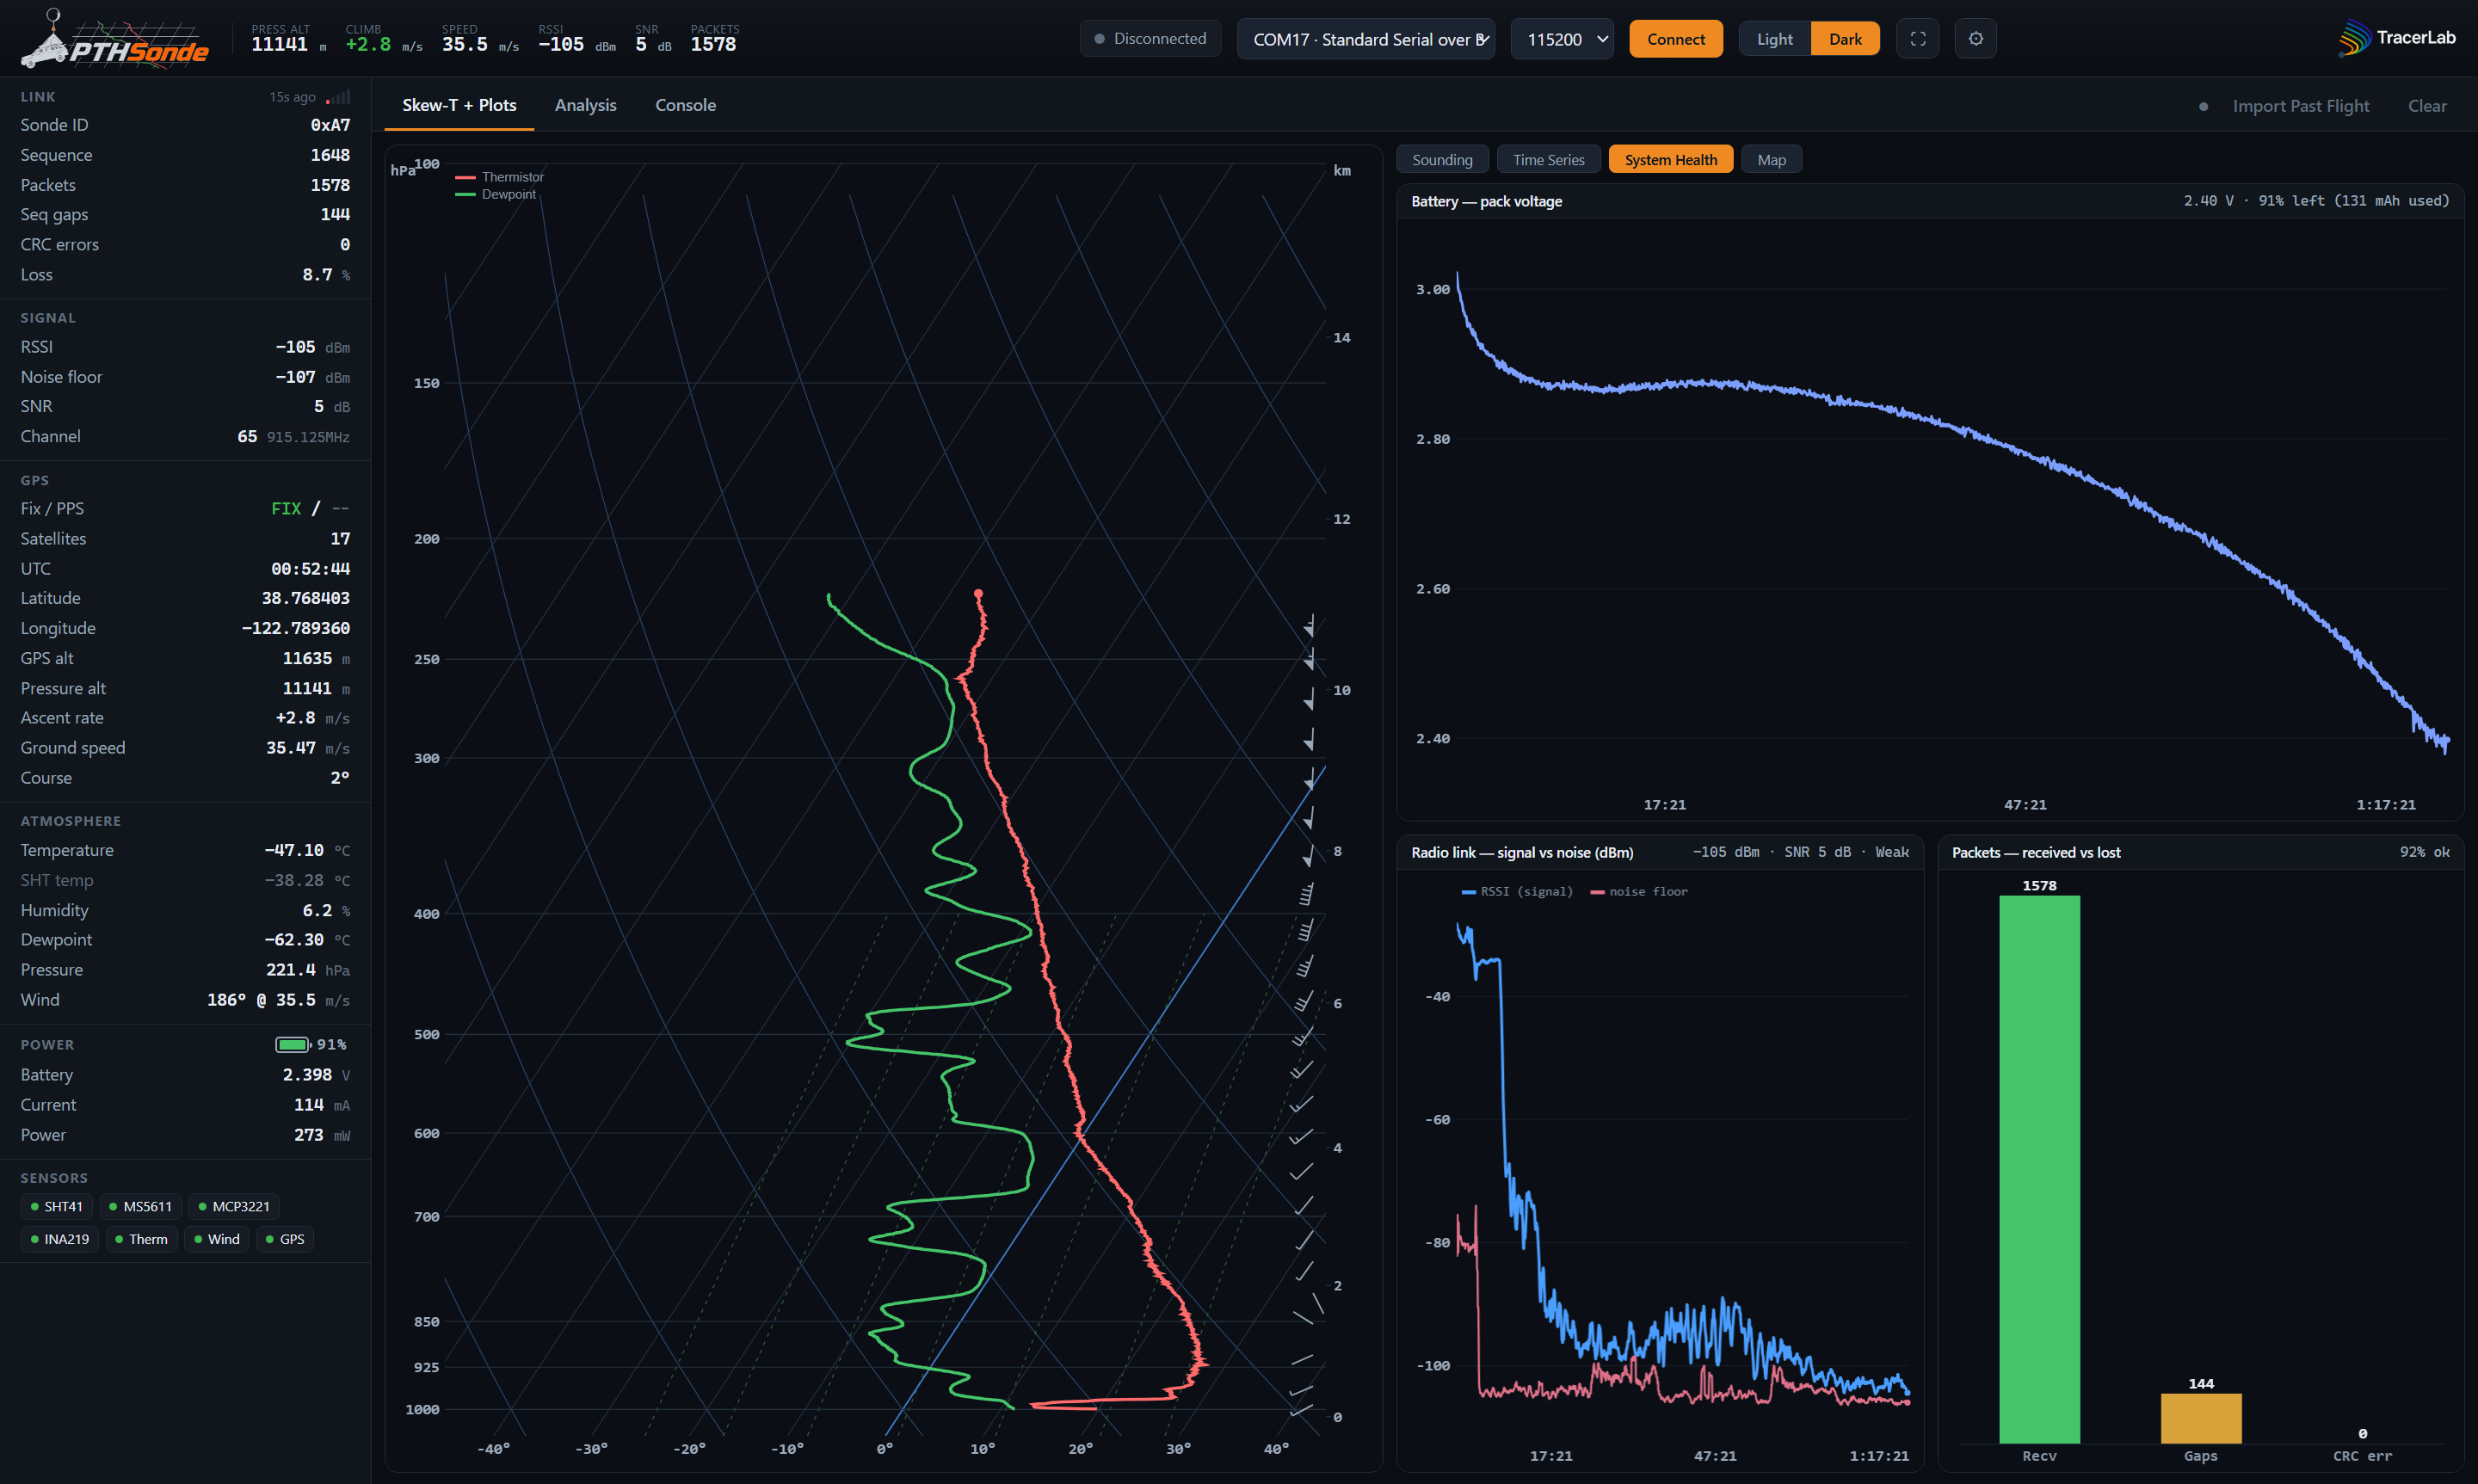
\includegraphics[width=\textwidth]{dash_health.png}
\caption{\textbf{System Health} view --- engineering telemetry (battery, current, RSSI/SNR,
sequence gaps) to confirm the payload is behaving.}
\end{figure}

\section{The flight predictor}
On the \textbf{Map} view, the \textbf{Flight Sim} button opens the landing predictor.
It fetches winds-aloft from a public GFS model for your launch point and time, then
flies a virtual balloon up and back down through those winds to estimate where the
payload will land --- \emph{before} you launch, and continuously refined during the
flight.

\begin{figure}[htbp]
\centering
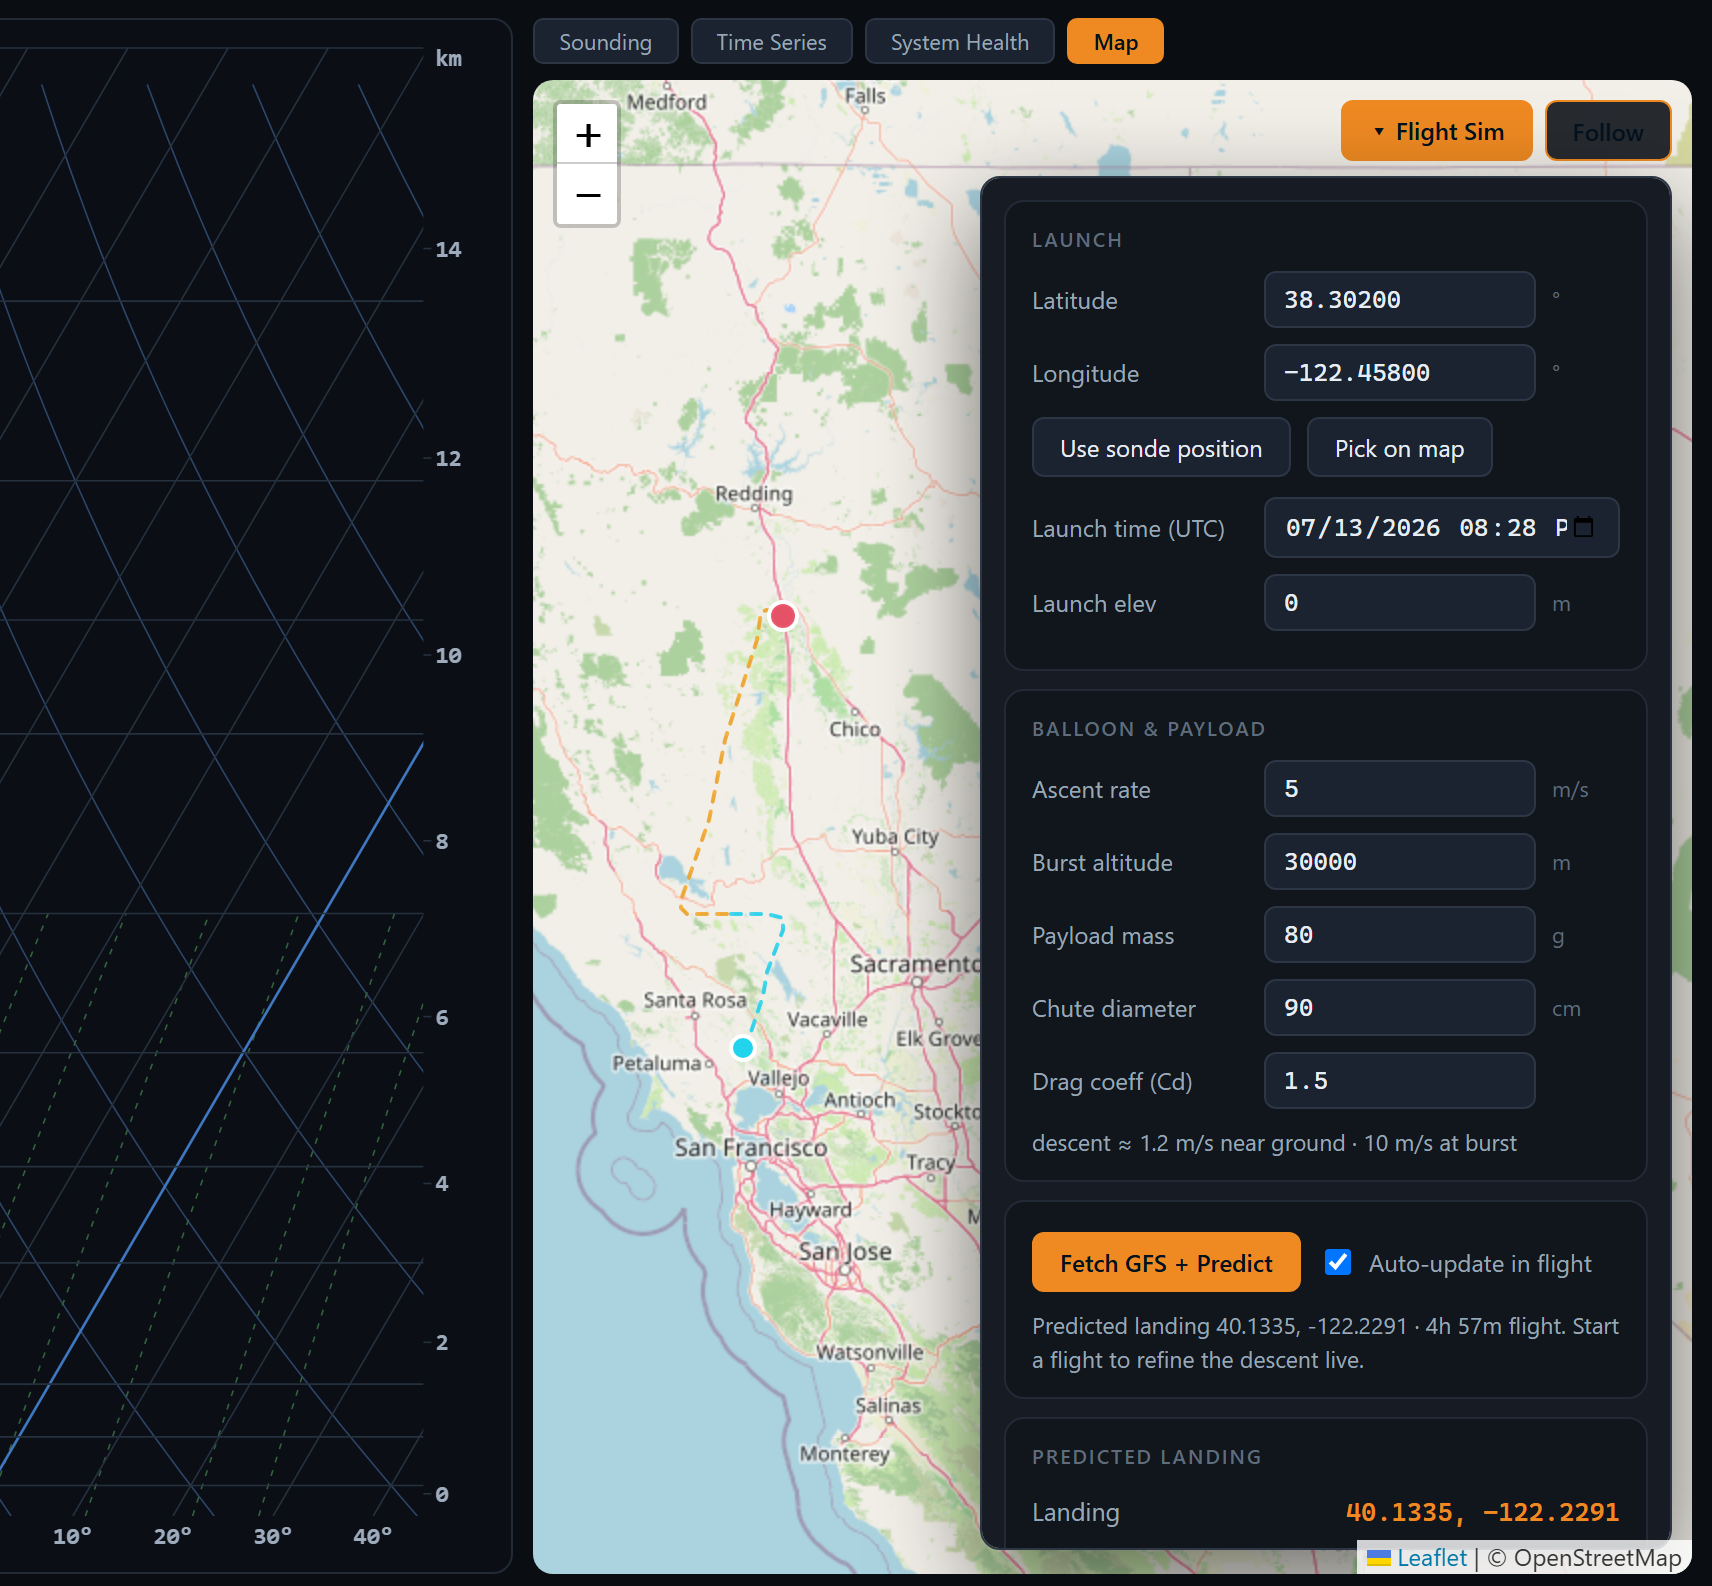
\includegraphics[width=0.64\textwidth]{dash_predictor.png}
\caption{The flight predictor. Set the launch point (type it, use the sonde's position,
or pick on the map) and your balloon numbers; the tool fetches GFS winds and draws the
predicted ascent (cyan), descent (orange) and landing (red), with a full flight summary.}
\end{figure}

\noindent To run a prediction:
\begin{enumerate}
  \item Set the \textbf{launch point} --- type a latitude/longitude, press
        \textbf{Use sonde position}, or \textbf{Pick on map}. Set the launch time and
        elevation (elevation defaults to $0$\,m).
  \item Enter the \textbf{balloon \& payload} numbers: ascent rate, burst altitude,
        payload mass, parachute diameter and drag coefficient. If you used the Fill
        Calculator, \textbf{Send to Flight Predictor} fills these for you.
  \item Press \textbf{Fetch GFS + Predict}. The map draws the trajectory and the panel
        reports the landing point, distance and bearing, burst altitude, time to burst,
        descent duration, total flight time and landing ETA.
\end{enumerate}

\begin{note}
Leave \textbf{Auto-update in flight} on and the prediction sharpens continuously as the
sonde flies --- it substitutes your balloon's own measured winds for the model winds at
every altitude you have already flown, so the landing estimate tightens on the way up.
\end{note}

\begin{tip}
Start the prediction \emph{before} you launch to make sure the forecast landing zone is
safe, reachable and clear of hazards and controlled airspace. A prediction needs an
internet connection to fetch the GFS winds.
\end{tip}

% =============================================================================
\chapter{Filling \& Preparing the Balloon}

The balloon lifts the 80\,g payload at a controlled rate to a controlled burst
altitude. Two numbers set the flight: how much gas you put in
(the \emph{lift}) and which balloon you fly.

\section{The physics of lift}
A balloon floats because the helium inside weighs less than the air it displaces.
At sea level, every litre of helium provides about
\[
  \text{net lift} \;=\; \rho_{\text{air}} - \rho_{\text{He}}
  \;=\; 1.225 - 0.179 \;\approx\; \mathbf{1.05\ \text{grams per litre}}.
\]
Three quantities matter when filling:
\begin{description}[leftmargin=1.5cm,style=nextline]
  \item[Gross lift] the total upward buoyancy of the gas.
  \item[Neck (nozzle) lift] gross lift minus the balloon's own weight --- this is what
        you \emph{measure} while filling, by hanging a known weight on the neck.
  \item[Free lift] neck lift minus the payload --- the net force that actually drives
        the ascent and sets the climb rate.
\end{description}
The standard target is a \textbf{5\,m/s ascent}: fast enough for a predictable
recovery window, slow enough for high-resolution data and a high burst.

\section{Choosing the balloon and filling it}
Two things set the flight: which balloon you fly, and how much gas you put in.

\subsection{The two standard balloons}
\begin{itemize}
  \item \textbf{50\,g balloon} --- small, less gas. Bursts around 12\,km. Good for a
        quick tropospheric profile and a nearby recovery.
  \item \textbf{150\,g balloon} --- reaches roughly 20\,km, deep into the stratosphere,
        for a full sounding. Needs more gas and covers more ground before landing.
\end{itemize}

The fill table gives the numbers for both, assuming the 80\,g \PTH{} train, a
5\,m/s target ascent and a drag coefficient $C_d=0.30$. \textbf{Fill until the balloon
just lifts a weight equal to the neck lift}, then attach the payload. Hydrogen lifts a
little more per litre, so it needs slightly less gas.

\begin{table}[H]
\centering\small
\renewcommand{\arraystretch}{1.3}
\begin{tabular}{@{}l cc cc@{}}
\toprule
 & \multicolumn{2}{c}{\textbf{50\,g balloon}} & \multicolumn{2}{c}{\textbf{150\,g balloon}} \\
\cmidrule(lr){2-3}\cmidrule(lr){4-5}
 & Helium & Hydrogen & Helium & Hydrogen \\
\midrule
Free lift                 & 325\,g & 294\,g & 407\,g & 370\,g \\
\rowcolor{tlorange!12}
\textbf{Neck (fill) lift} & \textbf{405\,g} & \textbf{374\,g} & \textbf{487\,g} & \textbf{450\,g} \\
Gas volume                & 435\,L & 373\,L & 608\,L & 529\,L \\
\quad(cubic feet)         & 15\,ft$^3$ & 13\,ft$^3$ & 21\,ft$^3$ & 19\,ft$^3$ \\
Launch diameter           & 0.9\,m & 0.9\,m & 1.05\,m & 1.0\,m \\
Approx.\ burst altitude   & 12\,km & 13\,km & 20\,km & 21\,km \\
\bottomrule
\end{tabular}
\caption{Recommended fill for the 80\,g \PTH{} train, for helium and hydrogen. Burst
altitudes assume typical burst diameters (1.5\,m for the 50\,g, 2.6\,m for the 150\,g) and
vary with the actual balloon batch.}
\end{table}

\begin{note}
\textbf{Recommended balloons: Kaymont.} Kaymont sounding balloons are a reliable,
widely-available choice with consistent, well-documented burst diameters --- fly the
50\,g or 150\,g size to match the profiles above.
\end{note}

\begin{tip}
\textbf{How to measure neck lift.} The cleanest method is a \textbf{spring scale}
(a fishing or luggage scale): anchor it to the ground, clip the balloon neck to it,
and add gas until the scale reads the neck-lift value from the table (e.g.\ 487\,g for
the 150\,g balloon on helium). Alternatively, tie a small container to the neck and add
water or weights until the total equals that value, then fill until the balloon
\emph{just} lifts the weight off the ground. Either way, you have exactly the right free
lift once the 80\,g payload replaces the weight.
\end{tip}

\begin{warn}
Use \textbf{helium}, not hydrogen, unless you are trained and equipped for it.
Fill outdoors or in a well-ventilated space, wear gloves, and never let the filled
balloon contact the ground or rough surfaces --- a nick becomes an early burst.
\end{warn}

\subsection{The Fill Calculator}
For any other balloon, gas, payload or target altitude, the dashboard's
\textbf{Fill Calculator} tab does the same physics interactively --- using the same
buoyancy-versus-drag model as the table above, so the numbers match.

\begin{figure}[H]
\centering
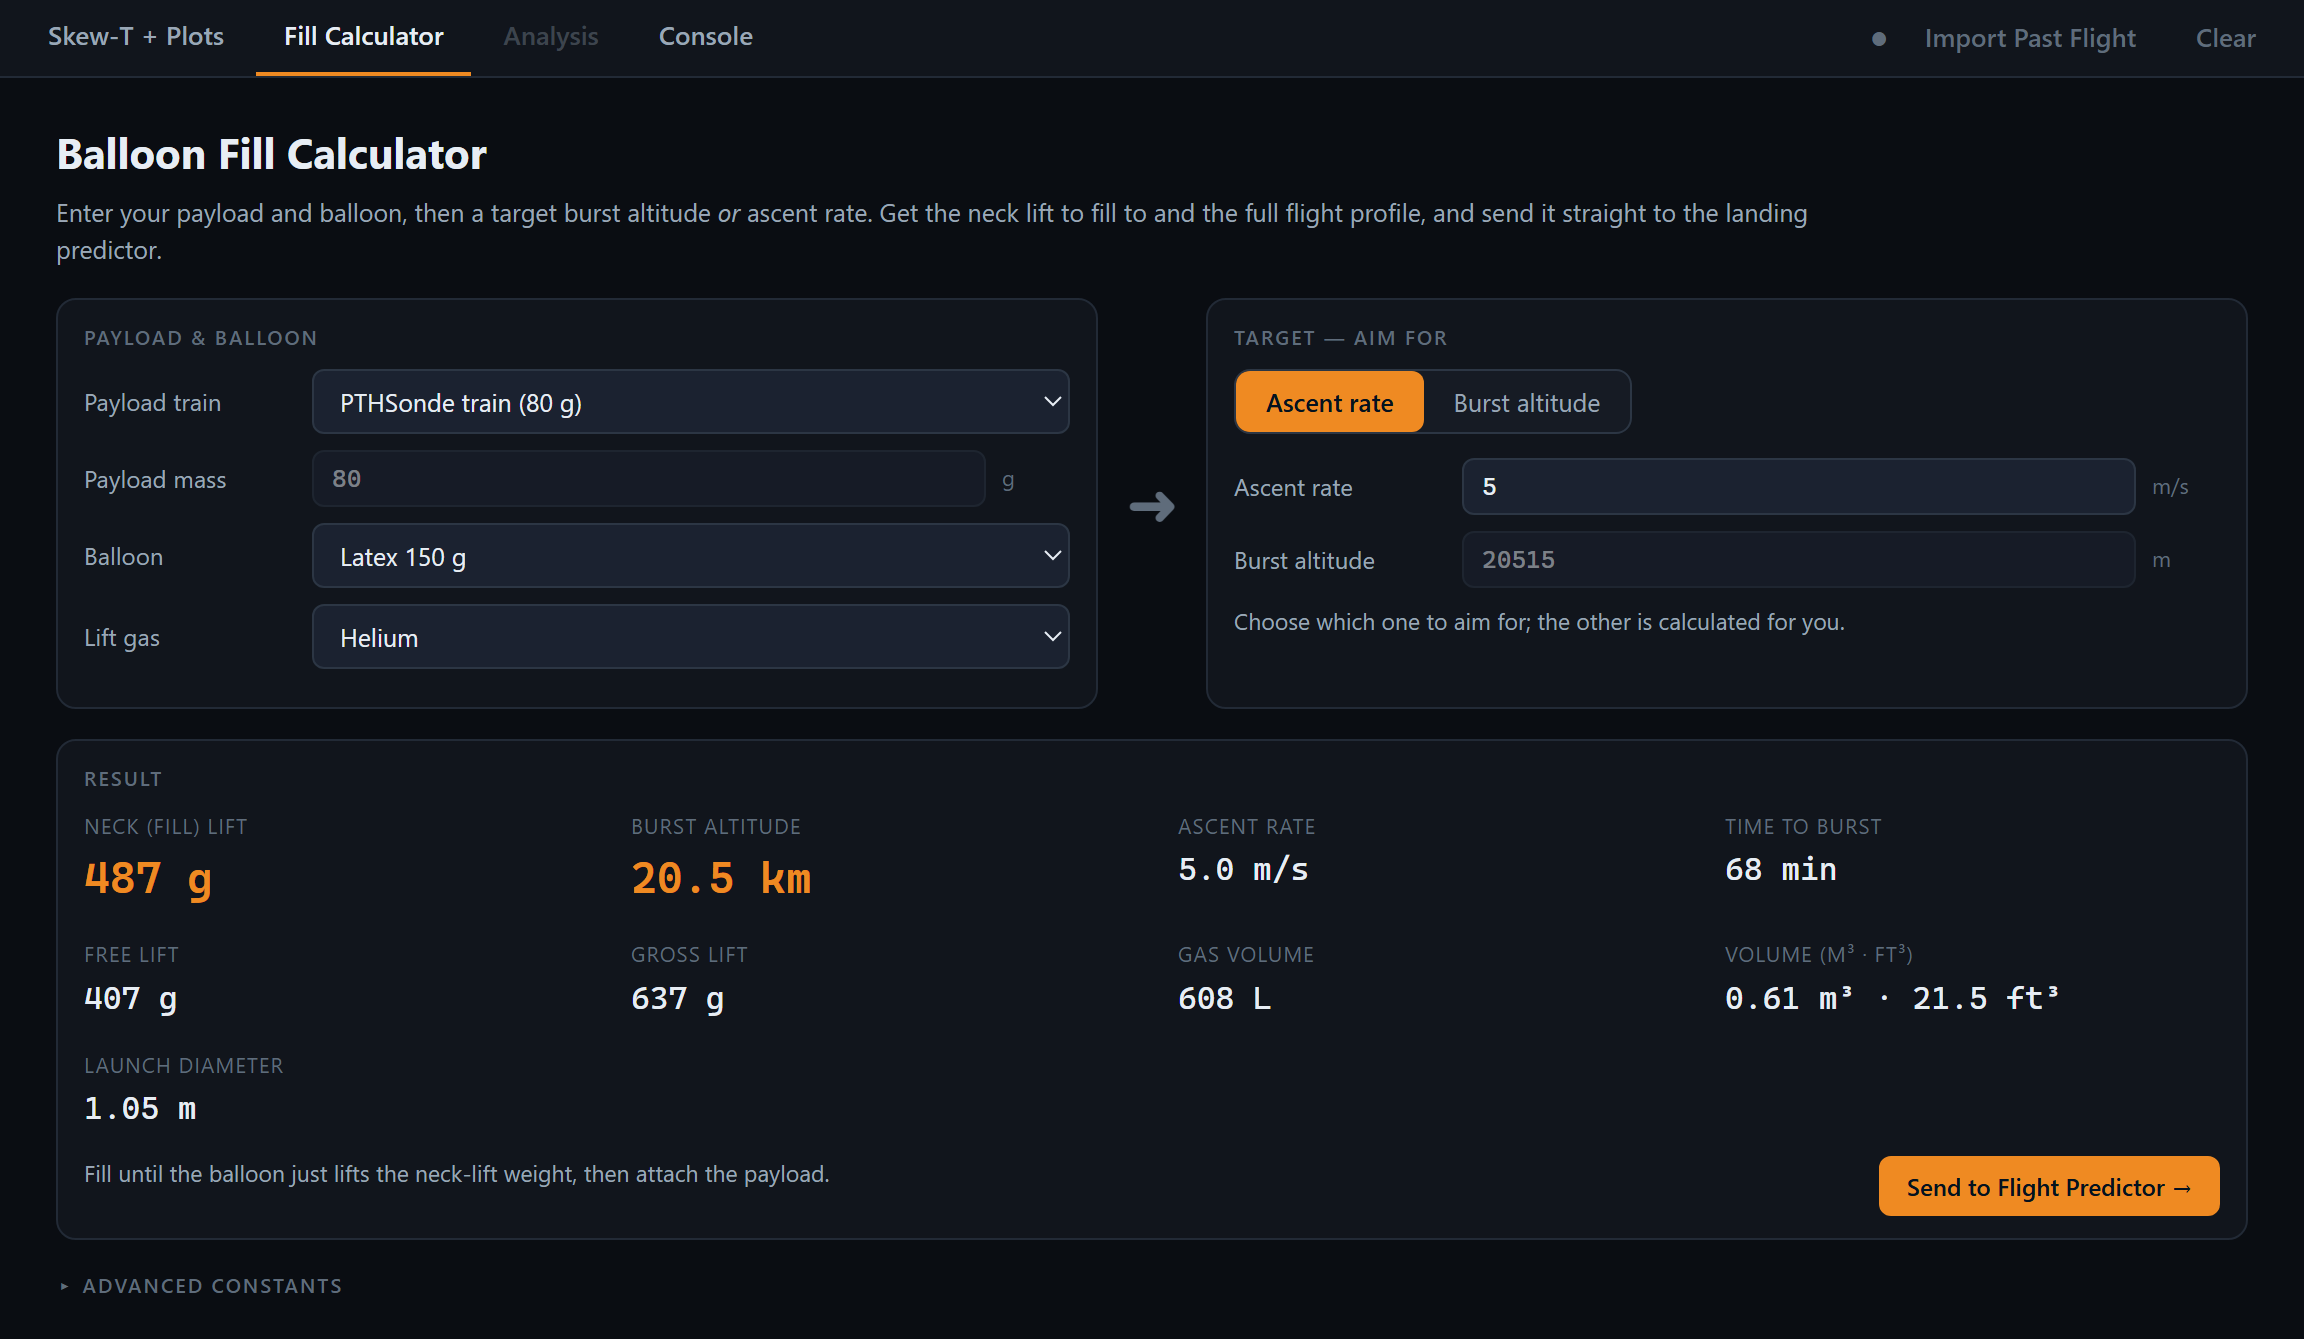
\includegraphics[width=0.98\textwidth]{dash_fillcalc.png}
\caption{The Fill Calculator. Choose the payload train and balloon, pick your gas, and
aim for either a target ascent rate or a target burst altitude --- it returns the neck
lift to fill to, the gas volume, launch diameter and the full flight profile.}
\end{figure}

\noindent To use it:
\begin{enumerate}
  \item Pick the \textbf{payload train} --- \textsc{PTHSonde train (80\,g)} locks the
        mass to the standard train, or choose \textsc{custom} to type your own.
  \item Choose the \textbf{balloon} from the manufacturer list (Kaymont/Totex, Hwoyee,
        Pawan, or the \PTH{} 50\,g / 150\,g latex) and the \textbf{lift gas}
        (helium, hydrogen, and others). The balloon's mass and burst diameter fill in
        automatically; a \textsc{custom} balloon lets you set them under
        \emph{Advanced constants}.
  \item Under \textbf{Target}, choose whether to aim for an \textbf{ascent rate} or a
        \textbf{burst altitude}; the other is calculated for you.
  \item Read off the \textbf{neck (fill) lift} --- the weight to hang on the neck while
        filling --- along with the gas volume, launch diameter, burst altitude and time
        to burst. \textbf{Send to Flight Predictor} carries these straight to the
        landing predictor (Chapter~4).
\end{enumerate}

\begin{note}
Burst diameters in the balloon list are manufacturer nominal values and vary with
batch, temperature and fill. Treat every result as a planning estimate and confirm your
neck lift by measurement before launch.
\end{note}

\clearpage
\section{Assembling the flight train}
Rig the train top-to-bottom so everything hangs in a straight line below the balloon.

\begin{figure}[H]
\centering
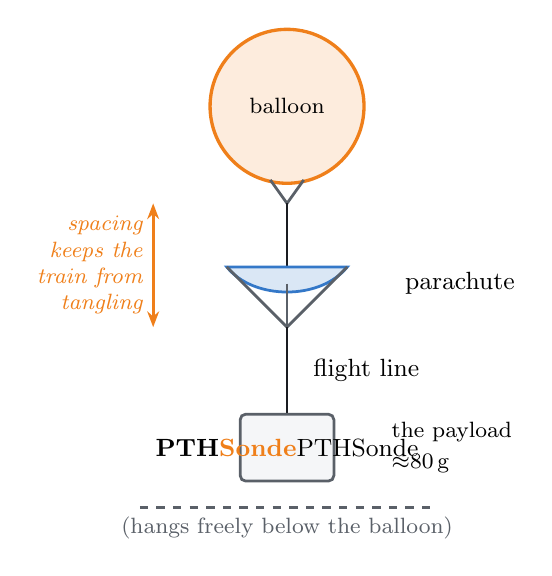
\begin{tikzpicture}[font=\small,line width=1pt,scale=0.85]
  % balloon
  \draw[fill=tlorange!15,draw=tlorange,line width=1.2pt] (0,7) circle (1.15);
  \node at (0,7) {\footnotesize balloon};
  \draw[tlgray] (-0.25,5.9) -- (0,5.55) -- (0.25,5.9); % neck
  % line to parachute
  \draw[tldark] (0,5.55) -- (0,4.6);
  % parachute
  \draw[fill=tlblue!18,draw=tlblue,line width=1pt] (-0.9,4.6) .. controls (-0.5,4.1) and (0.5,4.1) .. (0.9,4.6) -- cycle;
  \draw[tlgray] (-0.9,4.6) -- (0,3.7); \draw[tlgray] (0.9,4.6) -- (0,3.7); \draw[tlgray] (0,4.35) -- (0,3.7);
  \node[right=6mm] at (0.9,4.35) {parachute};
  % flight line
  \draw[tldark] (0,3.7) -- (0,2.4);
  \node[right=2mm] at (0,3.05) {flight line};
  % sonde
  \draw[rounded corners=2pt,fill=tllight,draw=tlgray,line width=1pt] (-0.7,1.4) rectangle (0.7,2.4);
  \node at (0,1.9) {\PTH};
  \node[right=6mm,align=left] at (0.7,1.9) {\footnotesize the payload\\\footnotesize $\approx$80\,g};
  % ground
  \draw[tlgray,dashed] (-2.2,1.0) -- (2.2,1.0);
  \node[tlgray] at (0,0.7) {\footnotesize (hangs freely below the balloon)};

  % dimension bracket
  \draw[{Stealth[length=2mm]}-{Stealth[length=2mm]},tlorange] (-2.0,5.55) -- node[left,align=right,font=\footnotesize\itshape]{spacing\\keeps the\\train from\\tangling} (-2.0,3.7);
\end{tikzpicture}
\caption{The flight train, top to bottom: balloon, parachute, flight line, and the \PTH{}
payload. The parachute rides between the balloon and the payload so it deploys on burst.}
\end{figure}

% =============================================================================
\chapter{Launching}

\section{Pre-launch checklist}
\begin{enumerate}
  \item Sonde battery fresh; door zip-tied; all sensor dots green on the dashboard.
  \item Sonde \textbf{locked} onto the flight channel; packets arriving with good RSSI.
  \item GPS has a fix (satellite count climbing) with a clear view of the sky.
  \item Balloon filled to the correct neck lift; neck tied off twice; parachute rigged.
  \item Flight line knots inspected; payload hanging clean.
  \item Recovery gear ready; landing-prediction map checked for a safe drift.
\end{enumerate}

\section{Release}
Pick a moment with light, steady surface wind. Walk the payload downwind of the
balloon so the train is stretched out, then release the balloon and let the line
lift the payload smoothly out of your hand --- never throw it.

\begin{figure}[htbp]
\centering
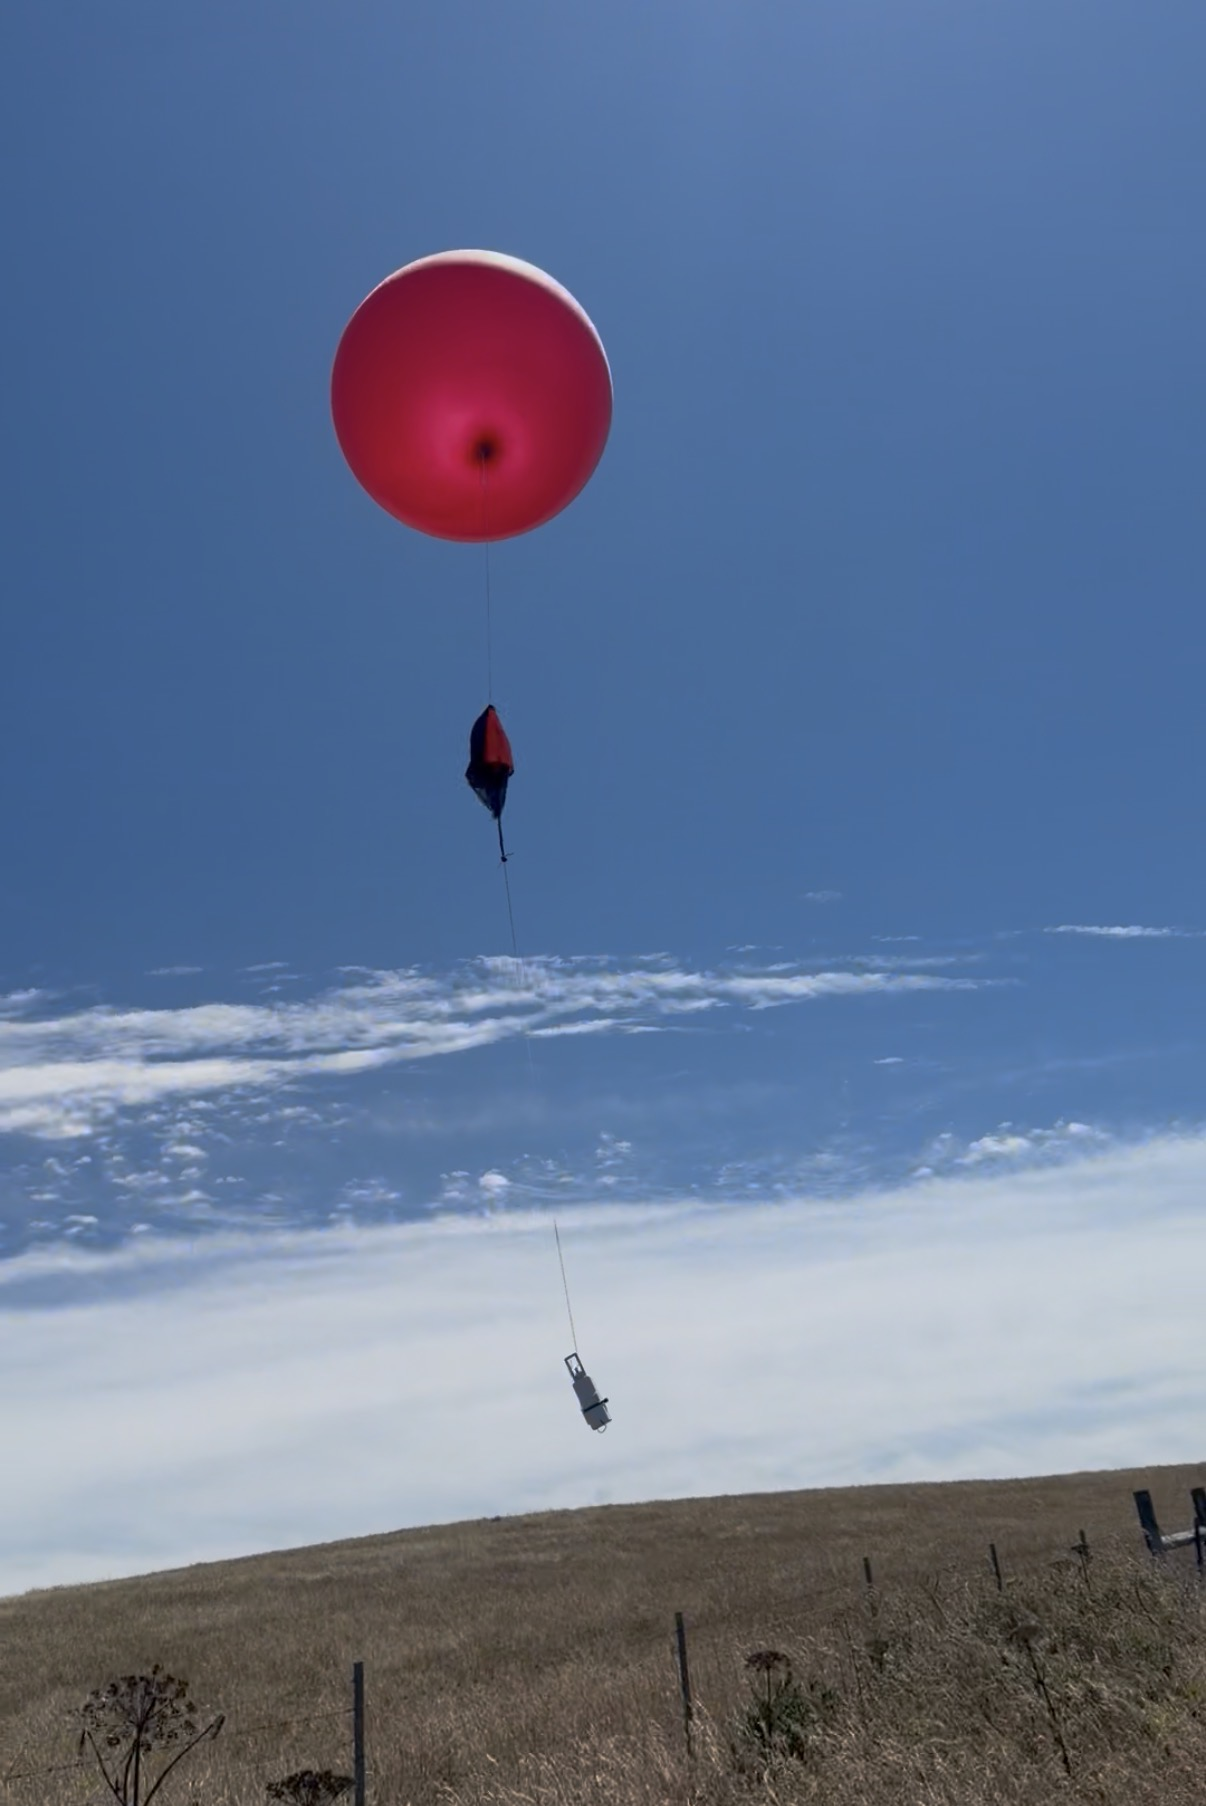
\includegraphics[width=0.7\textwidth]{launch.jpg}
\caption{Release. Let the balloon lift the flight line and payload cleanly out of your hands;
the dashboard should immediately show the climb rate go positive.}
\end{figure}

\begin{tip}
The instant the sonde leaves the ground the dashboard's \textsc{climb} number should
jump to roughly $+5$\,m/s and the pressure altitude should start rising. If it does
not climb, you are under-filled --- bring it back and add gas.
\end{tip}

% =============================================================================
\chapter{In-Flight Operations \& Data}

\section{Tracking the flight}
Once airborne, the dashboard shows the complete flight picture:
\begin{itemize}
  \item The \textbf{Skew-T} builds up in real time as the sonde climbs through the atmosphere.
  \item The \textbf{Map} shows the current position and the predicted landing point for recovery.
  \item The \textbf{header} tells you altitude, climb rate and link health at a glance.
  \item At burst the climb rate flips sharply negative; the parachute then controls the descent.
\end{itemize}

\section{Recording \& processing}
The app records every packet to a flight folder on disk as it arrives. When the
flight ends, one click processes the recording: it cleans the profile, and renders
the SHARPpy sounding panel from your own data.

\begin{note}
Because altitude and ascent rate are derived from the barometric pressure sensor,
the profile keeps building even after the GPS reaches its altitude ceiling --- the
sounding is complete all the way to burst.
\end{note}

% =============================================================================
\chapter{SHARPpy Sounding Analysis}

The primary product of a flight is a SHARPpy SPC panel, rendered from the
balloon's own temperature, humidity and wind profile. It turns raw telemetry into
the same Skew-T / hodograph / index panel meteorologists use operationally.

\begin{figure}[htbp]
\centering
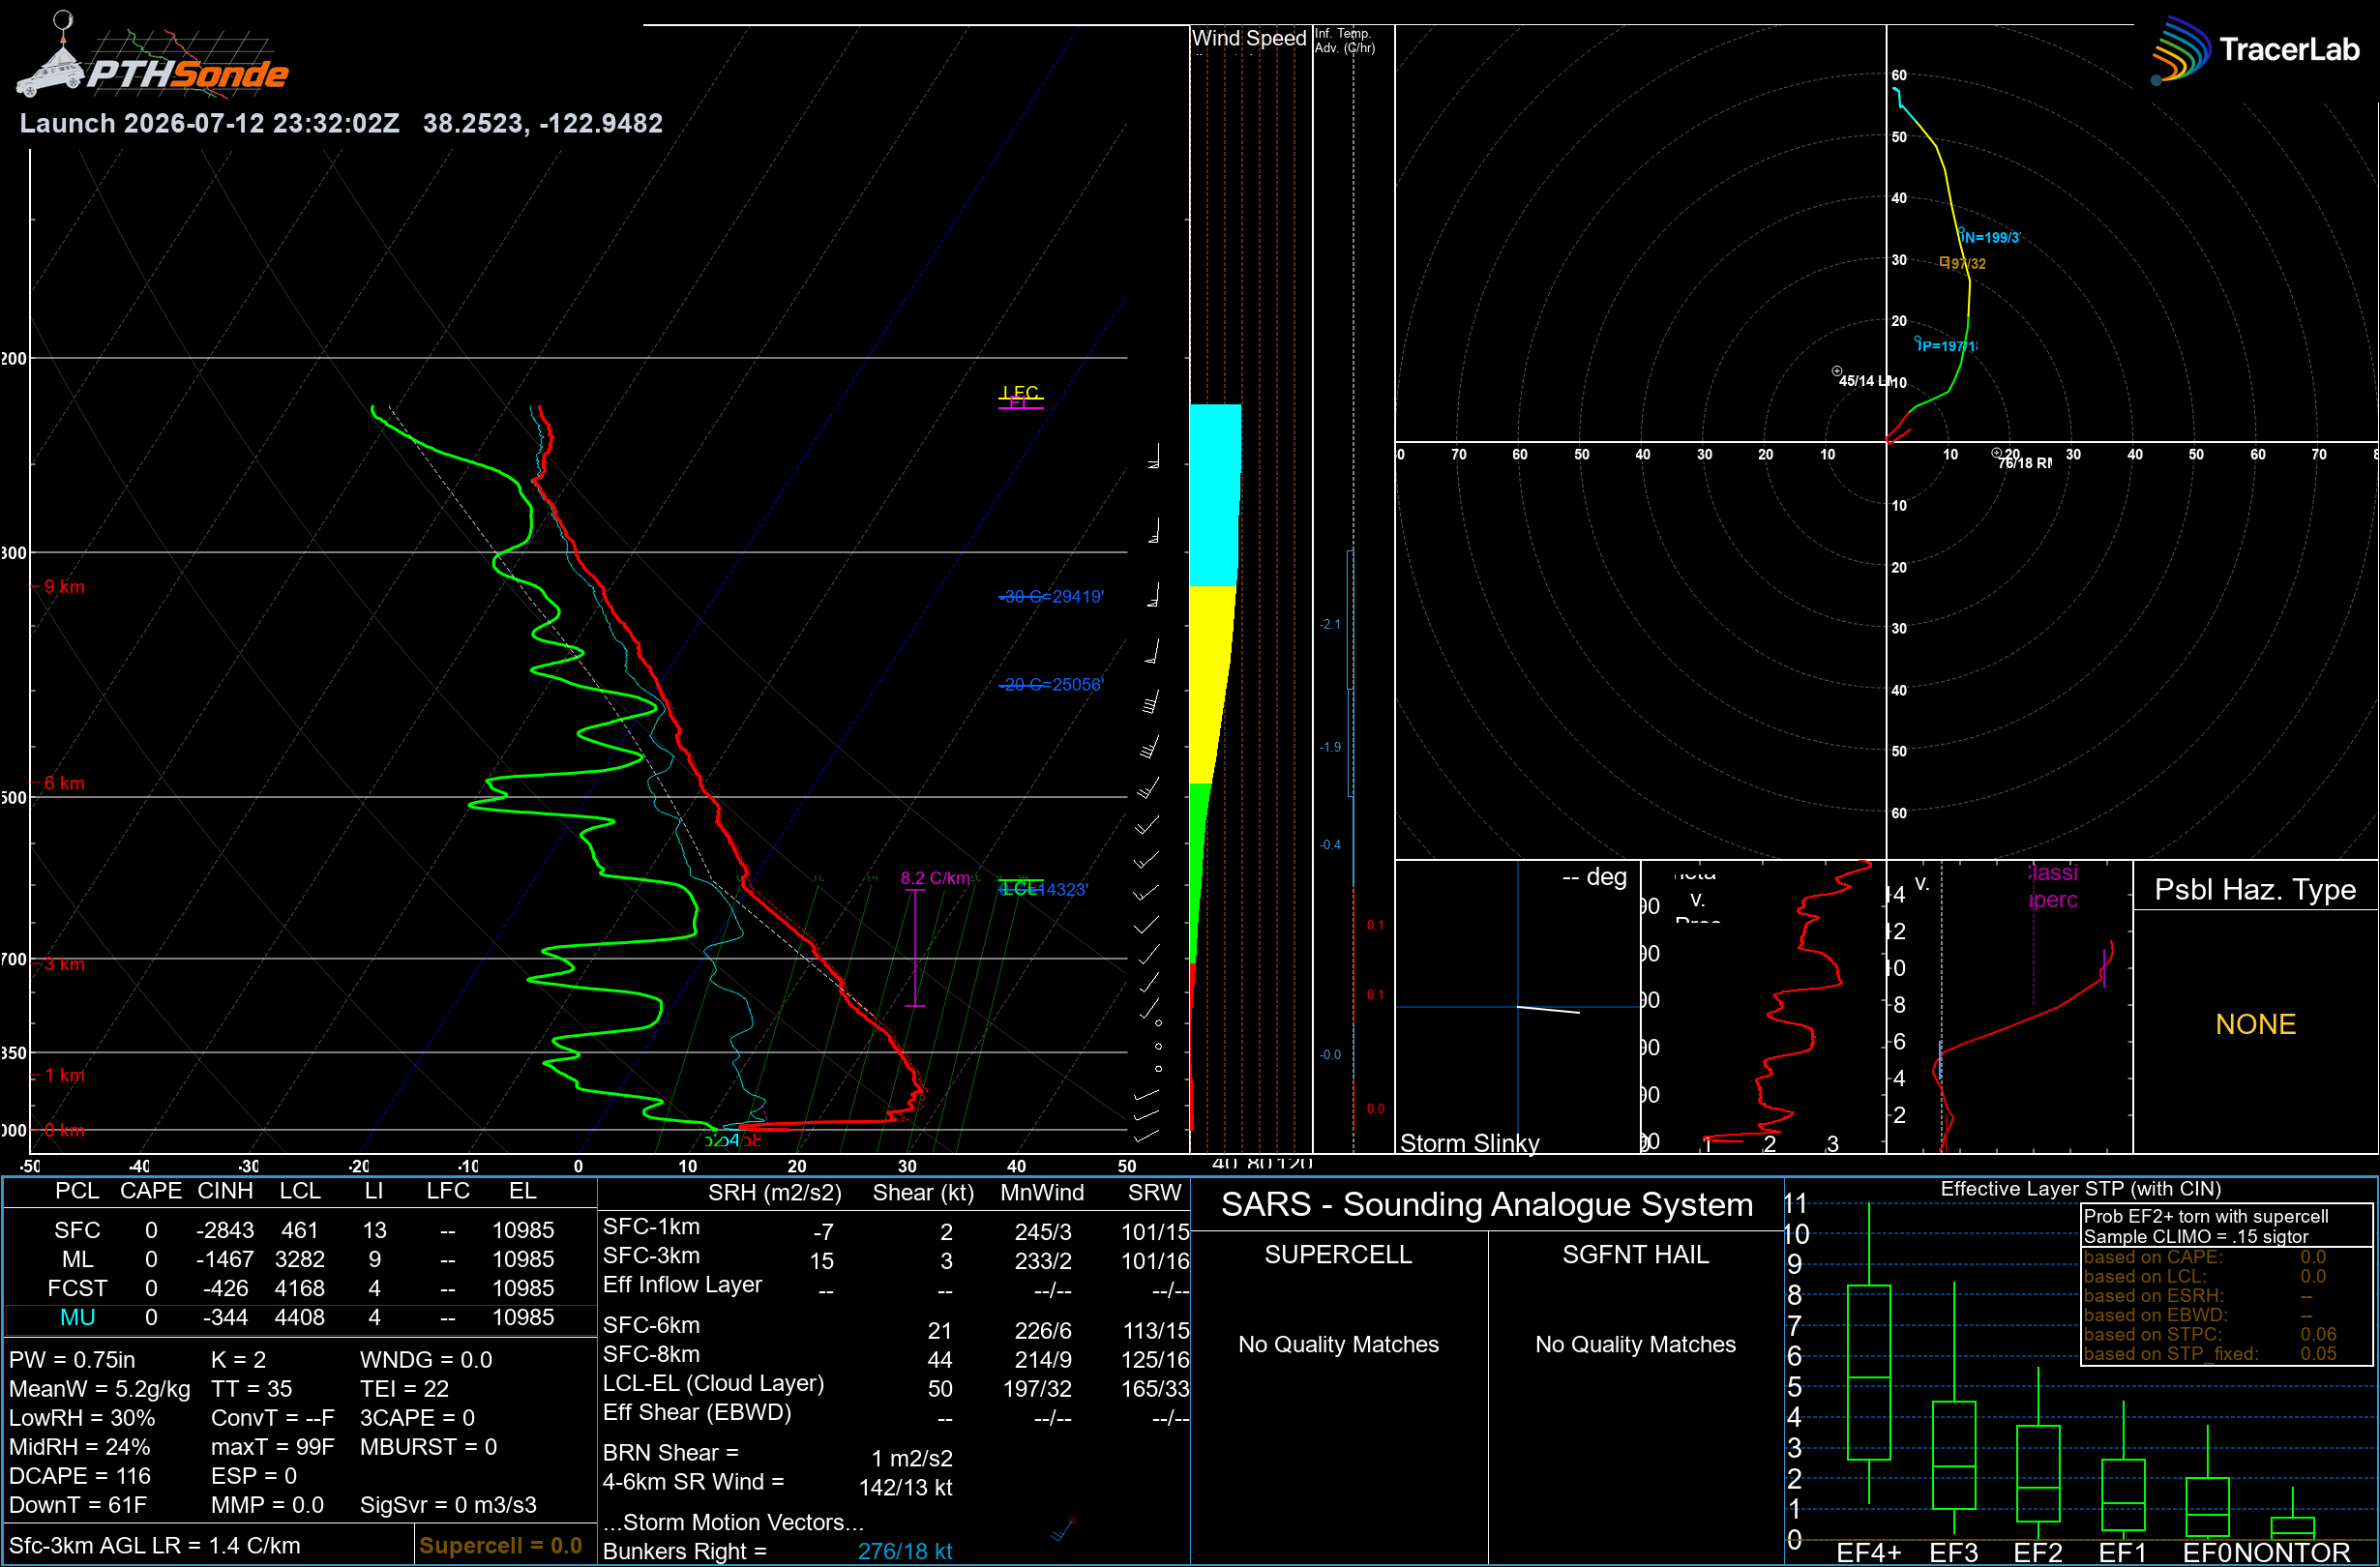
\includegraphics[width=\textwidth]{sharppy_example.png}
\caption{Example SHARPpy panel from a \PTH{} flight. The Skew-T (left) shows the temperature and
dewpoint profile with the lifted parcel path; the hodograph (upper right) shows the wind with
height; and the tables report the standard convective and kinematic indices.}
\end{figure}

\section{Reading the panel --- every value defined}
The panel presents a complete severe-weather analysis in one view. Each quantity it
reports is described below, grouped by what it tells you --- and, for each index, gives
its typical value \emph{scale} and a representative \emph{example} inline, so you can
read a number and know immediately what it means. The examples are drawn from one
coherent illustrative sounding: a moderately unstable, well-sheared spring afternoon ---
the classic supercell setup. A quiet day (like the calm flight shown earlier) would read
near zero across the instability and severe indices; contrast the two to build intuition.

\subsection{The plots}
\begin{description}[leftmargin=3.4cm,style=nextline]
  \item[Skew-T log-P] The environmental temperature (right curve) and dewpoint (left curve)
        versus pressure on skewed axes. The dashed line is the lifted-parcel path; area where the
        parcel is warmer than the environment is CAPE, where cooler is CIN. Their left--right
        separation is the dryness of the air.
  \item[Hodograph] The horizontal wind vector traced with height. Its length is the bulk shear;
        its curvature is the storm-relative helicity --- both key to storm organisation.
  \item[Storm Slinky] A 3-D cartoon of the modelled updraft's shape and tilt --- a quick visual of
        how sheared the environment is.
  \item[Inferred Temp.\ Advection] Warm- or cold-air advection through the column, inferred from how
        the wind veers (warm) or backs (cold) with height.
\end{description}

\subsection{Lifted-parcel indices (the PCL table)}
Each row lifts a different starting parcel: \textbf{SFC} (from the surface),
\textbf{ML} (the average of the lowest 100\,hPa, ``mixed layer''), \textbf{FCST} (a
forecast surface parcel at the expected afternoon high), and \textbf{MU} (the
most-unstable parcel, highest $\theta_e$). For each parcel:
\begin{description}[leftmargin=2.2cm,style=nextline]
  \item[CAPE] Convective Available Potential Energy (J/kg) --- the buoyant energy available to the
        parcel, the energy that drives updrafts. \emph{Scale:} $0$ none $\cdot$ $<\!1000$ weak $\cdot$
        $1000$--$2500$ moderate $\cdot$ $2500$--$4000$ strong $\cdot$ $>\!4000$ extreme.
        \emph{Example:} $2500$\,J/kg = strong instability.
  \item[CINH] Convective Inhibition (J/kg) --- the negative-buoyancy ``cap'' that must be overcome
        before free convection. \emph{Scale:} $0$ to $-25$ weak (easily broken) $\cdot$ $-25$ to
        $-100$ moderate $\cdot$ $<\!-100$ strong cap. \emph{Example:} $-45$ = moderate, breakable
        by afternoon heating.
  \item[LCL] Lifted Condensation Level (m) --- the height cloud base forms. \emph{Scale:} lower is
        more tornado-favorable; $<\!1000$\,m low $\cdot$ $>\!2000$\,m high/dry.
        \emph{Example:} $900$\,m = low, favorable.
  \item[LFC] Level of Free Convection (m) --- the height above which the parcel is freely buoyant;
        the lower it is, the more readily storms initiate. \emph{Example:} $1500$\,m.
  \item[EL] Equilibrium Level (m) --- where the parcel stops being buoyant, roughly the cloud/anvil
        top; higher means deeper storms. \emph{Example:} $12000$\,m = deep convection.
  \item[LI] Lifted Index ($^\circ$C) --- parcel-minus-environment temperature at 500\,hPa; negative
        means an unstable, storm-prone airmass. \emph{Scale:} $>\!0$ stable $\cdot$ $0$ to $-3$
        marginal $\cdot$ $-3$ to $-6$ moderate $\cdot$ $-6$ to $-9$ very unstable $\cdot$ $<\!-9$
        extreme. \emph{Example:} $-7\,^\circ$C = very unstable.
\end{description}

\subsection{Thermodynamic \& moisture indices}
\begin{description}[leftmargin=2.6cm,style=nextline]
  \item[PW] Precipitable Water (in) --- total column water vapour. \emph{Scale:} $<\!0.5$ very dry
        $\cdot$ $0.5$--$1.0$ average $\cdot$ $1.0$--$1.5$ moist $\cdot$ $>\!1.5$ heavy-rain
        potential. \emph{Example:} $1.3$\,in = moist.
  \item[MeanW] Mean water-vapour mixing ratio (g/kg) of the boundary layer; higher is moister.
        \emph{Example:} $14$\,g/kg = a rich, moist boundary layer.
  \item[LowRH / MidRH] Mean relative humidity (\%) of the low and mid levels. Moist low over dry
        mid favours strong downdrafts. \emph{Example:} $80\%/45\%$.
  \item[K-Index] Thunderstorm potential from mid-level temperature and moisture. \emph{Scale:}
        $<\!20$ unlikely $\cdot$ $20$--$25$ isolated $\cdot$ $26$--$30$ scattered $\cdot$ $31$--$35$
        numerous $\cdot$ $>\!35$ likely/heavy. \emph{Example:} $32$ = numerous.
  \item[Total Totals] Severe-storm index combining low-level moisture and the mid-level lapse rate.
        \emph{Scale:} $<\!44$ weak $\cdot$ $44$--$50$ strong $\cdot$ $50$--$55$ severe likely $\cdot$
        $>\!55$ intense. \emph{Example:} $52$ = severe likely.
  \item[Sfc--3km LR] Temperature lapse rate over the lowest 3\,km ($^\circ$C/km); steeper is more
        unstable. $\sim\!7$--$8\,^\circ$C/km is steep. \emph{Example:} $7.5\,^\circ$C/km.
  \item[ConvT] Convective Temperature --- the surface temperature needed to break the cap; compare
        it to maxT to see if storms will fire. \emph{Example:} $29\,^\circ$C.
  \item[maxT] Forecast daytime maximum temperature. \emph{Example:} $31\,^\circ$C (above ConvT ---
        cap breaks).
  \item[3CAPE] CAPE in the lowest 3\,km --- low-level updraft strength, relevant to tornadoes;
        $>\!100$\,J/kg is meaningful. \emph{Example:} $120$\,J/kg.
  \item[DCAPE] Downdraft CAPE (J/kg) --- energy available to downdrafts; gust/outflow potential.
        \emph{Scale:} $<\!500$ weak $\cdot$ $500$--$1000$ moderate gusts $\cdot$ $>\!1000$ strong
        outflow / microburst. \emph{Example:} $900$\,J/kg.
  \item[DownT] Estimated downdraft (wet-bulb) surface temperature --- the cool outflow.
        \emph{Example:} $18\,^\circ$C.
\end{description}

\subsection{Kinematic (wind) indices}
\begin{description}[leftmargin=2.6cm,style=nextline]
  \item[Shear] Bulk wind difference across a layer (kt), e.g.\ SFC--1\,km, SFC--6\,km, SFC--8\,km;
        organises storms. \emph{0--6\,km scale:} $<\!20$ single-cell $\cdot$ $20$--$35$ multicell /
        marginal supercell $\cdot$ $35$--$50$ supercell $\cdot$ $>\!50$ strong supercell.
        \emph{Example:} $55$\,kt = strong deep-layer shear.
  \item[Eff Shear / EBWD] Effective Bulk Wind Difference --- bulk shear over the storm's effective
        inflow layer; supercell range is $\sim\!35$--$50\!+$\,kt. \emph{Example:} $50$\,kt.
  \item[SRH] Storm-Relative Helicity (m$^2$/s$^2$), 0--1\,km and 0--3\,km --- the streamwise
        vorticity a storm can ingest; rotation/tornado potential. \emph{0--1\,km scale:} $<\!100$
        low $\cdot$ $100$--$150$ supercell possible $\cdot$ $150$--$300$ tornadic-favorable $\cdot$
        $>\!300$ strong. \emph{Example:} $250$\,m$^2$/s$^2$.
  \item[SRW] Storm-Relative Wind --- the wind a moving storm ``sees'' in a given layer; stronger
        means better updraft ventilation. \emph{Example:} $30$\,kt (0--2\,km).
  \item[MnWind] Mean wind over a layer --- overall steering flow.
  \item[BRN Shear] The shear term of the Bulk Richardson Number --- pairs instability with shear.
  \item[Bunkers R / L] Predicted right- and left-moving supercell storm-motion vectors; use them to
        drive to the storm / recovery. \emph{Example:} R at $240^\circ / 35$\,kt.
\end{description}

\subsection{Composite severe-weather indices}
\begin{description}[leftmargin=2.6cm,style=nextline]
  \item[SigSvr] Significant Severe parameter (ML CAPE $\times$ 0--6\,km shear); higher means more
        significant severe. \emph{Example:} $60{,}000$ = well into the significant-severe range.
  \item[Supercell] Supercell Composite Parameter --- CAPE, shear and helicity combined into a
        supercell likelihood. \emph{Scale:} $<\!1$ non-supercell $\cdot$ $1$--$4$ possible $\cdot$
        $>\!4$ strong supercell. \emph{Example:} $8$ = strong.
  \item[STP] Significant Tornado Parameter (effective-layer, CIN-weighted); the EF-scale bars show
        analogue tornado probabilities. \emph{Scale:} $<\!1$ unlikely $\cdot$ $1$--$2$ possible
        $\cdot$ $>\!2$ favorable for significant tornadoes. \emph{Example:} $3$.
  \item[WNDG] Wind Damage Parameter --- potential for damaging convective winds; $>\!1$ is elevated.
        \emph{Example:} $1.5$.
  \item[ESP] Enhanced Stretching Potential --- low-level stretching for landspout/weak-tornado
        potential. \emph{Example:} $0.5$.
  \item[MMP] MCS Maintenance Probability ($0$--$1$) --- whether an organised storm complex can
        sustain itself. \emph{Example:} $0.6$.
  \item[TEI] Theta-E Index --- mid-level dryness / downdraft potential; higher means drier aloft.
        \emph{Example:} $30$.
  \item[MBURST] Microburst composite --- wet/dry microburst potential. \emph{Example:} $4$.
  \item[SARS] Sounding Analogue System --- matches your profile to historical significant-hail and
        supercell soundings. \emph{Example:} matches sig-hail / supercell analogues.
  \item[Poss.\ Hazard Type] SHARPpy's one-line overall verdict for the sounding --- e.g.\
        \textsc{none}, \textsc{mrgl}, or \textsc{tor} on a tornado-capable day.
\end{description}

% =============================================================================
\chapter{Appendix}

\section{Downlink telemetry}
Each transmission is a compact, CRC-checked binary packet sent a few times per
minute. It carries the sonde ID and sequence, UTC time, GPS position and altitude,
pressure, temperature, humidity, thermistor temperature, battery voltage/current,
and status/validity flags. Wind is derived on the ground from successive GPS fixes.

\section{Quick reference}
\begin{table}[htbp]
\centering\small
\begin{tabular}{@{}>{\bfseries}l l@{}}
\toprule
Parameter & Typical value \\
\midrule
Radio band & 915\,MHz ISM (LoRa) \\
Transmit power & 22\,dBm \\
Flight train mass & $\approx$80\,g \\
Target ascent rate & 5\,m/s \\
Neck lift, 50\,g balloon & $\approx$365\,g \\
Neck lift, 150\,g balloon & $\approx$450\,g \\
Burst altitude, 50\,g / 150\,g & $\approx$11\,km / $\approx$20\,km \\
Helium net lift & $\approx$1.05\,g/L \\
\bottomrule
\end{tabular}
\caption{At-a-glance operating figures for the \PTH{} system.}
\end{table}

\vfill
\begin{center}

\includegraphics[width=0.28\textwidth]{logo_tracerlab.png}\\[4pt]
{\color{tlgray}\small \PTH{} --- Tracer Lab}
\end{center}

\end{document}
